
%\documentclass[11pts,a4paper,amsmath,amssymb,floatfix]{article}%{report}%{book}
\documentclass[12pts,a4paper,amsmath,amssymb,floatfix]{article}%{report}%{book}
\usepackage{graphicx,wrapfig}% Include figure files
%\usepackage{dcolumn,enumerate}% Align table columns on decimal point
\usepackage{enumerate,enumitem}% Align table columns on decimal point
\usepackage{bm,dpfloat}% bold math
\usepackage[pdftex,bookmarks,colorlinks=true,urlcolor=rltblue,citecolor=blue]{hyperref}
\usepackage{amsfonts,amsmath,amssymb,stmaryrd,indentfirst}
\usepackage{times,psfrag}
\usepackage{natbib}
\usepackage{color}
\usepackage{units}
\usepackage{rotating}
\usepackage{multirow}

\usepackage{pifont}
\usepackage{subfigure}
\usepackage{subeqnarray}
\usepackage{ifthen} 
  
\usepackage{supertabular} 
\usepackage{moreverb}
\usepackage{fancyvrb}
\usepackage{listings}  
\usepackage{palatino} 
%\usepackage{doi}
\usepackage{longtable} 
\usepackage{float}
\usepackage{perpage,comment}
\MakeSorted{figure}
%\usepackage{pdflscape}

\definecolor{rltblue}{rgb}{0,0,0.75}

 
%\usepackage{natbib}
\usepackage{fancyhdr} %%%%
\pagestyle{fancy}%%%%
% with this we ensure that the chapter and section
% headings are in lowercase
%%%%\renewcommand{\chaptermark}[1]{\markboth{#1}{}}
\renewcommand{\sectionmark}[1]{\markright{\thesection\ #1}}
\fancyhf{} %delete the current section for header and footer
\fancyhead[LE,RO]{\bfseries\thepage}
\fancyhead[LO]{\bfseries\rightmark}
\fancyhead[RE]{\bfseries\leftmark}
\renewcommand{\headrulewidth}{0.5pt}
% make space for the rule
\fancypagestyle{plain}{%
\fancyhead{} %get rid of the headers on plain pages
\renewcommand{\headrulewidth}{0pt} % and the line
}

\def\newblock{\hskip .11em plus .33em minus .07em}
\usepackage{color}

%\usepackage{makeidx}
%\makeindex

\setlength\textwidth      {16.cm}
\setlength\textheight     {22.6cm}
\setlength\oddsidemargin  {-0.3cm}
\setlength\evensidemargin {0.3cm}

\setlength\headheight{14.49998pt} 
\setlength\topmargin{0.0cm}
\setlength\headsep{1.cm}
\setlength\footskip{1.cm}
\setlength\parskip{0pt} 
\setlength\parindent{0pt} 

%%% 
%%% Headers and Footers
\lhead[] {\text{\small{EG3521 -- Engineering Thermodynamics}}} 
%\chead[] {\text{\small{Session 2012/13}}}  
\lfoot[]{Module 03}  
%\cfoot[\thepage]{\thepage}
\rfoot[\text{\small{\thepage}}]{\thepage}
\rhead[] {{\text{\small{Session 2013/14}}}}
\renewcommand{\headrulewidth}{0.8pt}
 
%%% 
%%% space between lines
%%%
\renewcommand{\baselinestretch}{1.5}

\newenvironment{VarDescription}[1]%
  {\begin{list}{}{\renewcommand{\makelabel}[1]{\textbf{##1:}\hfil}%
    \settowidth{\labelwidth}{\textbf{#1:}}%
    \setlength{\leftmargin}{\labelwidth}\addtolength{\leftmargin}{\labelsep}}}%
  {\end{list}}

%%%%%%%%%%%%%%%%%%%%%%%%%%%%%%%%%%%%%%%%%%%
%%%%%%                              %%%%%%%
%%%%%%      NOTATION SECTION        %%%%%%%
%%%%%%                              %%%%%%%
%%%%%%%%%%%%%%%%%%%%%%%%%%%%%%%%%%%%%%%%%%%

% Text abbreviations.
\newcommand{\ie}{{\em{i.e., }}}
\newcommand{\eg}{{\em{e.g., }}}
\newcommand{\cf}{{\em{cf., }}}
\newcommand{\wrt}{with respect to}
\newcommand{\lhs}{left hand side}
\newcommand{\rhs}{right hand side}
% Commands definining mathematical notation.

% This is for quantities which are physically vectors.
\renewcommand{\vec}[1]{{\mbox{\boldmath$#1$}}}
% Physical rank 2 tensors
\newcommand{\tensor}[1]{\overline{\overline{#1}}}
% This is for vectors formed of the value of a quantity at each node.
\newcommand{\dvec}[1]{\underline{#1}}
% This is for matrices in the discrete system.
\newcommand{\mat}[1]{\mathrm{#1}}


\DeclareMathOperator{\sgn}{sgn}
\newtheorem{thm}{Theorem}[section]
\newtheorem{lemma}[thm]{Lemma}

%\newcommand\qed{\hfill\mbox{$\Box$}}
\newcommand{\re}{{\mathrm{I}\hspace{-0.2em}\mathrm{R}}}
\newcommand{\inner}[2]{\langle#1,#2\rangle}
\renewcommand\leq{\leqslant}
\renewcommand\geq{\geqslant}
\renewcommand\le{\leqslant}
\renewcommand\ge{\geqslant}
\renewcommand\epsilon{\varepsilon}
\newcommand\eps{\varepsilon}
\renewcommand\phi{\varphi}
\newcommand{\bmF}{\vec{F}}
\newcommand{\bmphi}{\vec{\phi}}
\newcommand{\bmn}{\vec{n}}
\newcommand{\bmns}{{\textrm{\scriptsize{\boldmath $n$}}}}
\newcommand{\bmi}{\vec{i}}
\newcommand{\bmj}{\vec{j}}
\newcommand{\bmk}{\vec{k}}
\newcommand{\bmx}{\vec{x}}
\newcommand{\bmu}{\vec{u}}
\newcommand{\bmv}{\vec{v}}
\newcommand{\bmr}{\vec{r}}
\newcommand{\bma}{\vec{a}}
\newcommand{\bmg}{\vec{g}}
\newcommand{\bmU}{\vec{U}}
\newcommand{\bmI}{\vec{I}}
\newcommand{\bmq}{\vec{q}}
\newcommand{\bmT}{\vec{T}}
\newcommand{\bmM}{\vec{M}}
\newcommand{\bmtau}{\vec{\tau}}
\newcommand{\bmOmega}{\vec{\Omega}}
\newcommand{\pp}{\partial}
\newcommand{\kaptens}{\tensor{\kappa}}
\newcommand{\tautens}{\tensor{\tau}}
\newcommand{\sigtens}{\tensor{\sigma}}
\newcommand{\etens}{\tensor{\dot\epsilon}}
\newcommand{\ktens}{\tensor{k}}
\newcommand{\half}{{\textstyle \frac{1}{2}}}
\newcommand{\tote}{E}
\newcommand{\inte}{e}
\newcommand{\strt}{\dot\epsilon}
\newcommand{\modu}{|\bmu|}
% Derivatives
\renewcommand{\d}{\mathrm{d}}
\newcommand{\D}{\mathrm{D}}
\newcommand{\ddx}[2][x]{\frac{\d#2}{\d#1}}
\newcommand{\ddxx}[2][x]{\frac{\d^2#2}{\d#1^2}}
\newcommand{\ddt}[2][t]{\frac{\d#2}{\d#1}}
\newcommand{\ddtt}[2][t]{\frac{\d^2#2}{\d#1^2}}
\newcommand{\ppx}[2][x]{\frac{\partial#2}{\partial#1}}
\newcommand{\ppxx}[2][x]{\frac{\partial^2#2}{\partial#1^2}}
\newcommand{\ppt}[2][t]{\frac{\partial#2}{\partial#1}}
\newcommand{\pptt}[2][t]{\frac{\partial^2#2}{\partial#1^2}}
\newcommand{\DDx}[2][x]{\frac{\D#2}{\D#1}}
\newcommand{\DDxx}[2][x]{\frac{\D^2#2}{\D#1^2}}
\newcommand{\DDt}[2][t]{\frac{\D#2}{\D#1}}
\newcommand{\DDtt}[2][t]{\frac{\D^2#2}{\D#1^2}}
% Norms
\newcommand{\Ltwo}{\ensuremath{L_2} }
% Basis functions
\newcommand{\Qone}{\ensuremath{Q_1} }
\newcommand{\Qtwo}{\ensuremath{Q_2} }
\newcommand{\Qthree}{\ensuremath{Q_3} }
\newcommand{\QN}{\ensuremath{Q_N} }
\newcommand{\Pzero}{\ensuremath{P_0} }
\newcommand{\Pone}{\ensuremath{P_1} }
\newcommand{\Ptwo}{\ensuremath{P_2} }
\newcommand{\Pthree}{\ensuremath{P_3} }
\newcommand{\PN}{\ensuremath{P_N} }
\newcommand{\Poo}{\ensuremath{P_1P_1} }
\newcommand{\PoDGPt}{\ensuremath{P_{-1}P_2} }

\newcommand{\metric}{\tensor{M}}
\newcommand{\configureflag}[1]{\texttt{#1}}

% Units
\newcommand{\m}[1][]{\unit[#1]{m}}
\newcommand{\km}[1][]{\unit[#1]{km}}
\newcommand{\s}[1][]{\unit[#1]{s}}
\newcommand{\invs}[1][]{\unit[#1]{s}\ensuremath{^{-1}}}
\newcommand{\ms}[1][]{\unit[#1]{m\ensuremath{\,}s\ensuremath{^{-1}}}}
\newcommand{\mss}[1][]{\unit[#1]{m\ensuremath{\,}s\ensuremath{^{-2}}}}
\newcommand{\K}[1][]{\unit[#1]{K}}
\newcommand{\PSU}[1][]{\unit[#1]{PSU}}
\newcommand{\Pa}[1][]{\unit[#1]{Pa}}
\newcommand{\kg}[1][]{\unit[#1]{kg}}
\newcommand{\rads}[1][]{\unit[#1]{rad\ensuremath{\,}s\ensuremath{^{-1}}}}
\newcommand{\kgmm}[1][]{\unit[#1]{kg\ensuremath{\,}m\ensuremath{^{-2}}}}
\newcommand{\kgmmm}[1][]{\unit[#1]{kg\ensuremath{\,}m\ensuremath{^{-3}}}}
\newcommand{\Nmm}[1][]{\unit[#1]{N\ensuremath{\,}m\ensuremath{^{-2}}}}

% Dimensionless numbers
\newcommand{\dimensionless}[1]{\mathrm{#1}}
\renewcommand{\Re}{\dimensionless{Re}}
\newcommand{\Ro}{\dimensionless{Ro}}
\newcommand{\Fr}{\dimensionless{Fr}}
\newcommand{\Bu}{\dimensionless{Bu}}
\newcommand{\Ri}{\dimensionless{Ri}}
\renewcommand{\Pr}{\dimensionless{Pr}}
\newcommand{\Pe}{\dimensionless{Pe}}
\newcommand{\Ek}{\dimensionless{Ek}}
\newcommand{\Gr}{\dimensionless{Gr}}
\newcommand{\Ra}{\dimensionless{Ra}}
\newcommand{\Sh}{\dimensionless{Sh}}
\newcommand{\Sc}{\dimensionless{Sc}}


% Journals
\newcommand{\IJHMT}{{\it International Journal of Heat and Mass Transfer}}
\newcommand{\NED}{{\it Nuclear Engineering and Design}}
\newcommand{\ICHMT}{{\it International Communications in Heat and Mass Transfer}}
\newcommand{\NET}{{\it Nuclear Engineering and Technology}}
\newcommand{\HT}{{\it Heat Transfer}}   
\newcommand{\IJHT}{{\it International Journal for Heat Transfer}}

\newcommand{\frc}{\displaystyle\frac}

\newlist{ExList}{enumerate}{1}
\setlist[ExList,1]{label={\bf Example 1.} {\bf \arabic*}}

\newlist{ProbList}{enumerate}{1}
\setlist[ProbList,1]{label={\bf Problem 1.} {\bf \arabic*}}

%%%%%%%%%%%%%%%%%%%%%%%%%%%%%%%%%%%%%%%%%%%
%%%%%%                              %%%%%%%
%%%%%% END OF THE NOTATION SECTION  %%%%%%%
%%%%%%                              %%%%%%%
%%%%%%%%%%%%%%%%%%%%%%%%%%%%%%%%%%%%%%%%%%%


% Cause numbering of subsubsections. 
%\setcounter{secnumdepth}{8}
%\setcounter{tocdepth}{8}

\setcounter{secnumdepth}{4}%
\setcounter{tocdepth}{4}%

\includeonly{Examples_04_01}%,Examples_01_02,Examples_01_03}

\DeclareMathAlphabet{\mathpzc}{OT1}{pzc}{m}{it}

\begin{document}


%%%
%%%  First Page
%%%
\begin{comment}
\begin{titlepage}

\begin{center}
\bigskip
 
\vspace{4.cm}
\begin{center}
\resizebox{80mm}{!}{
\includegraphics[clip=true]{../FigBanner/UoALarge}}
\end{center}

\vspace{3.5cm}
\bigskip

{\bf {\huge  EG3521: Engineering Thermodynamics}} \\

\bigskip
{\bf {\huge Module 03: Refrigeration and Liquefaction}}\\
{\bf {\Large Examples and Problems}}
\bigskip
\vspace{5.cm}

{\bf {\Large Dr Jeff Gomes}}
\bigskip

{\bf{\Large  School of Engineering}}\\
\vspace{3cm}    

\bigskip 

{\bf {\large \today}}
\end{center}
 

\end{titlepage}
\end{comment}

\setcounter{page}{1}

\vfill

\pagebreak
%\tableofcontents
%\begin{Large}

%\section{Module 4: Refrigeration and Liquefaction}

%%%
%\section{Gas Refrigeration Cycles}

\begin{center}
\begin{tabular}{||c||}
\hline \hline
Thermodynamic Tables for the fluids used in this  \\
list can be found in any Textbook or be downloaded from \\
  \\
\href{https://highered.mcgraw-hill.com/sites/dl/free/0073529214/395307/appdxs1_2.pdf}{https://highered.mcgraw-hill.com/sites/dl/free/0073529214/395307/appdxs1$\_$2.pdf} \\
\hline\hline
\end{tabular}
\end{center}

\begin{enumerate}
%%%
%%% Saphiro 10.53 (7th Ed.)
%%% 
\item \label{Ex1} {\it In a Brayton refrigeration cycle with regenerative heat exchanger, air enters the compressor at -6.15$^{\text{o}}$C and 1.0 bar, and is compressed isentropically to 2.70 bar. The compressed air enters the regenerative heat exchanger at 26.85$^{\text{o}}$C and is cooled to -6.15$^{\text{o}}$C before entering the turbine where is expanded isentropically (Fig. \ref{Ex1:Fig}). If the refrigeration capacity is 15 tons, calculate:
\begin{enumerate}
\item volumetric flow rate at the compressor inlet $\left(\text{m}^{3}/\text{min}\right)$;
\item coefficient of performance.
\end{enumerate}
}


\begin{figure}[h]
\begin{center}
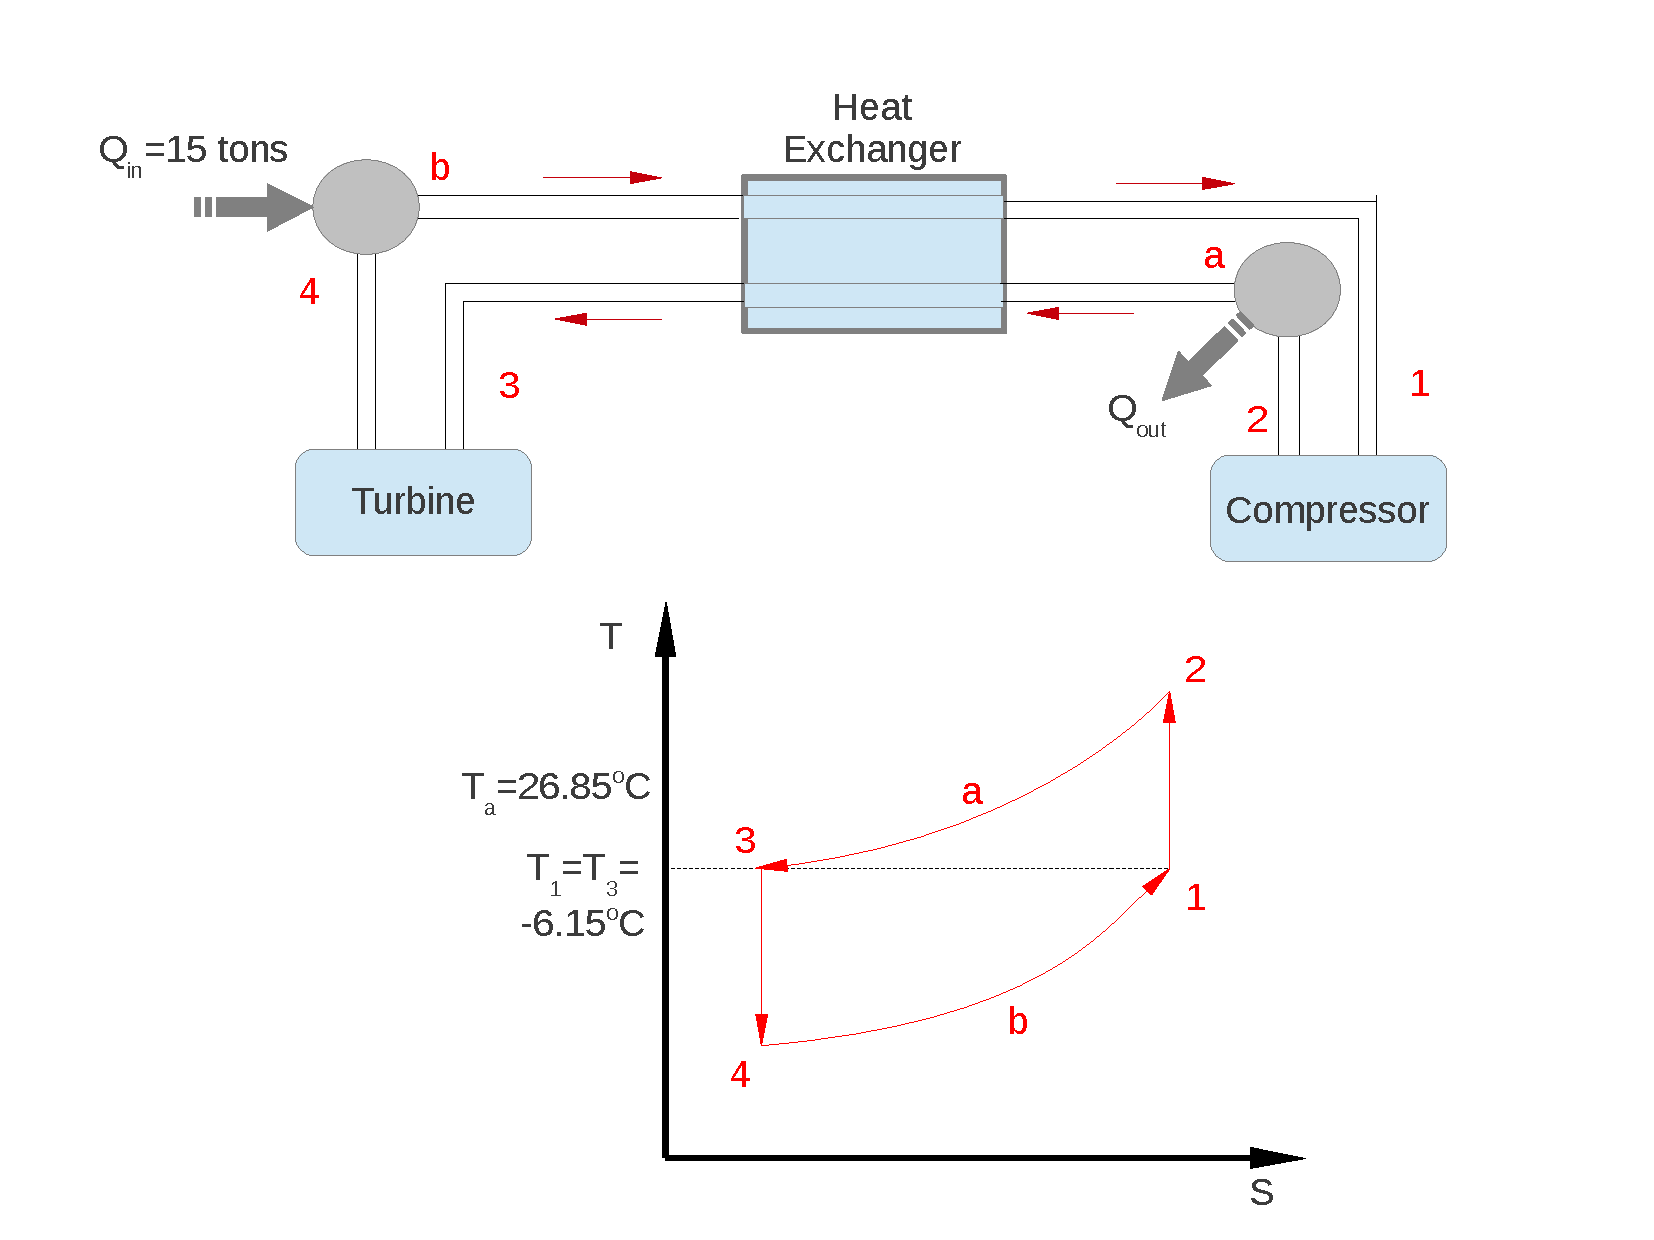
\includegraphics[width=13.0cm,height=10.0cm]{./Pics/Overview_Refrig11}
\end{center}
\caption{Gas refrigeration cycle: Problem \ref{Ex1}.}\label{Ex1:Fig}
\end{figure}

Let's first assume that there is no heat transfer from the heat exchanger to its surroundings. For each state shown in Fig. \ref{Ex1:Fig} we can extract the relevant data from the ideal gas properties of air tables\footnote{Moran, Shapiro, Boettner and Bailey; $\lq$Principles of Engineering Thermodynamics', Table A-22 (Seventh Edition).} 
\begin{itemize}
\item {\bf State 1:} At $T_{1}=-6.15^{\text{o}}\text{C}=267\text{ K}$ and $P_{1}=1$ bar\\
\begin{tabular}{ c c c }
{\bf T (K)} & {\bf H (kJ/kg)}  & {\bf P$_{r}$} \\
  260       &   260.09         &    0.8405  \\
  270       &   270.11         &    0.9590  \\
\end{tabular}

From linear interpolation $H_{1}$=267.10 kJ/kg and P$_{r,1}$=0.9235\footnote{Starting from the entropy definition, as a function of enthalpy and pressure, 
\begin{displaymath}
TdS=dH-VdP \rightarrow dS=\frc{dH}{T}-\frc{V}{T}dP
\end{displaymath}
Integrating the expression above from state 1 to state 2 and for ideal gas, $\frc{V}{T}=\frc{R}{P}$:
\begin{equation}
S\left(T_{2},P_{2}\right) - S\left(T_{1},P_{1}\right)=\int\limits_{T_{1}}^{T_{2}}C_{p}(T)\frc{dT}{T}-R\ln\frc{P_{2}}{P_{1}}\label{EqnEntropy}
\end{equation}
For an arbitrary reference temperature $\left(T_{r}\right)$ the second integral in the rhs can be rewritten as the integral difference:
\begin{displaymath}
\int\limits_{T_{1}}^{T_{2}}C_{p}\frc{dT}{T}=\int\limits_{T_{r}}^{T_{2}}C_{p}\frc{dT}{T} - \int\limits_{T_{r}}^{T_{1}}C_{p}\frc{dT}{T} = S^{\text{o}}\left(T_{2}\right)-S^{\text{o}}\left(T_{1}\right)
\end{displaymath}
where $S^{\text{o}}\left(T_{2}\right)$ and $S^{\text{o}}\left(T_{1}\right)$ depend {\bf only} on the temperature and can be easily tabulated in the same way as it is done for $H$ and $U$.  Thus for isentropic processes, Eqn. \ref{EqnEntropy} becomes
\begin{displaymath}
0 = S^{\text{o}}\left(T_{2}\right)-S^{\text{o}}\left(T_{1}\right) - R\ln\frc{P_{2}}{P_{1}}
\end{displaymath}
This equation can be easily manipulated,
\begin{displaymath}
\textcolor{red}{\frc{P_{2}}{P_{1}}} = \frc{\exp\left[S^{\text{o}}\left(T_{2}\right)/R\right]} {\exp\left[S^{\text{o}}\left(T_{1}\right)/R\right]} = \textcolor{red}{\frc{P_{r,2}}{P_{r,1}}}
\end{displaymath}
$P_{r}=P_{r}(T)$ is called {\it relative pressure}.}

\item {\bf State 2:} $P_{2}=2.80$ bar and as \textcolor{red}{1-2} is isentropic, we can use the {\it relative pressure} to calculate $H_{2}$,
\begin{displaymath}
\frc{P_{r,2}}{P_{r,1}} = \frc{P_{2}}{P_{1}} \Longrightarrow P_{r,2} = P_{r,1}\frc{P_{2}}{P_{1}} = 2.4935
\end{displaymath}
From the  ideal gas properties of air table,\\
\begin{tabular}{ c c c }
{\bf T (K)} & {\bf H (kJ/kg)}  & {\bf P$_{r}$} \\
  350       &   350.49         &    2.379  \\
  360       &   360.58         &    2.626  \\
\end{tabular}

$H_{2}=355.17$ kJ/kg, $T_{2}=354.63$ K$ = 81.48 ^{\text{o}}$C

\item {\bf State a:} $T_{a}=26.85^{\text{o}}$C$=300$ K $\Longrightarrow$ $H_{a}=300.19$ kJ/kg.

\item {\bf State 3:} $T_{3}=T_{1}=-6.15^{\text{o}}\text{C}=267\text{ K} \Longrightarrow$ $H_{3}$=267.10 kJ/kg and P$_{r,3}$=0.9235

\item {\bf State 4:} Similarly to state 2 and remembering that in Brayton cycles $P_{2}=P_{3}$ and $P_{1}=P_{4}$: 
\begin{displaymath}
P_{r,4} = P_{r,3}\frc{P_{4}}{P_{3}} = P_{r,3}\frc{P_{1}}{P_{2}} = 0.3420
\end{displaymath}
and from the ideal gas properties of air table, \\
\begin{tabular}{ c c c }
{\bf T (K)} & {\bf H (kJ/kg)}  & {\bf P$_{r}$} \\
  200       &   199.97         &    0.3363  \\
  210       &   209.97         &    0.3987 \\
\end{tabular}

From linear interpolation $H_{4}=200.88$ kJ/kg and $T_{4}=200.91$ K $= -72.24^{\text{o}}$C.

\item {\bf State b:} A simple energy balance in the heat exchanger (assuming that no heat is lost/gained to/from the surroundings)
\begin{displaymath}
\left(H_{b}-H_{1}\right) + \left(H_{a}-H_{3}\right) = 0 \Rightarrow H_{b} = -(300.19-267.10)+267.10 = 234.01 \text{ kJ/kg}
\end{displaymath}
\end{itemize}

With the given refrigeration capacity, the air mass flow rate is
\begin{displaymath}
\dot{m} = \frc{\dot{Q}_{in}}{\left(H_{b}-H_{4}\right)} = \frc{15 [tons]}{234.01-200.88 [kJ/kg]}\times \frc{1.4\times 10^{4}\;\;[kJ/h]}{1\;\;[ton]}=6338.67 \text{ kg/h}
\end{displaymath}
And the volumetric flow rate at the compressor intake is (molecular weight of dry air is 28.97 g/gmol):
\begin{eqnarray}
\textcolor{red}{\dot{V}} &=& \frc{\dot{m}RT_{1}}{P_{1}} = \frc{6338.67\left[\frc{kg}{h}\right] \times 8.314\times 10^{-5}\left[\frc{m^{3}.bar}{gmol.K}\right]\times 267\;[K]\times \left[\frc{1\;gmol}{28.97\;g}\right]\times \left[\frc{1000\;g}{1\;kg}\right]\times\frc{1\;[h]}{60\;[min]}}{1\;[bar]} \nonumber \\
&=& \textcolor{red}{80.95 \frc{\text{m}^{3}}{\text{min}}} \nonumber
\end{eqnarray}

The coefficient of performance (COP) is
\begin{displaymath}
\textcolor{red}{\text{COP}} = \frc{\text{Refrigerant Effect}}{\text{Work done}} = \frc{H_{b}-H_{4}}{\left(H_{2}-H_{1}\right)-\left(H_{3}-H_{4}\right)} = \frc{234.01 - 200.88}{(355.17-267.10)-(267.10-200.88)} = \textcolor{red}{1.516}
\end{displaymath}

%%%
%%% Saphiro 10.54 (7th Ed.)
%%% 
\item \label{Ex2} {\it Assume now that the compressor and turbine of  Problem \ref{Ex1} have isentropic efficiencies of 88$\%$. Answer the same questions for the modified cycle as in Problem \ref{Ex1}.}


%%%
%%% Saphiro 10.57 (7th Ed.)
%%% 
\item \label{Ex3}{\it  Air undergoes a Stirling refrigeration cycle. At the beginning of the isothermal compression, the pressure and temperature are 100 kPa and 300 K, respectively. The compression ratio is 6, and the temperature during the isothermal expansion is 100 K. Calculate:
\begin{enumerate}
\item The heat transfer during the isothermal expansion in kJ/kg of air;
\item The net work for the cycle in kJ/kg of air;
\item The coefficient of performance.
\end{enumerate}  
}

\begin{figure}[h]
 \begin{center}
  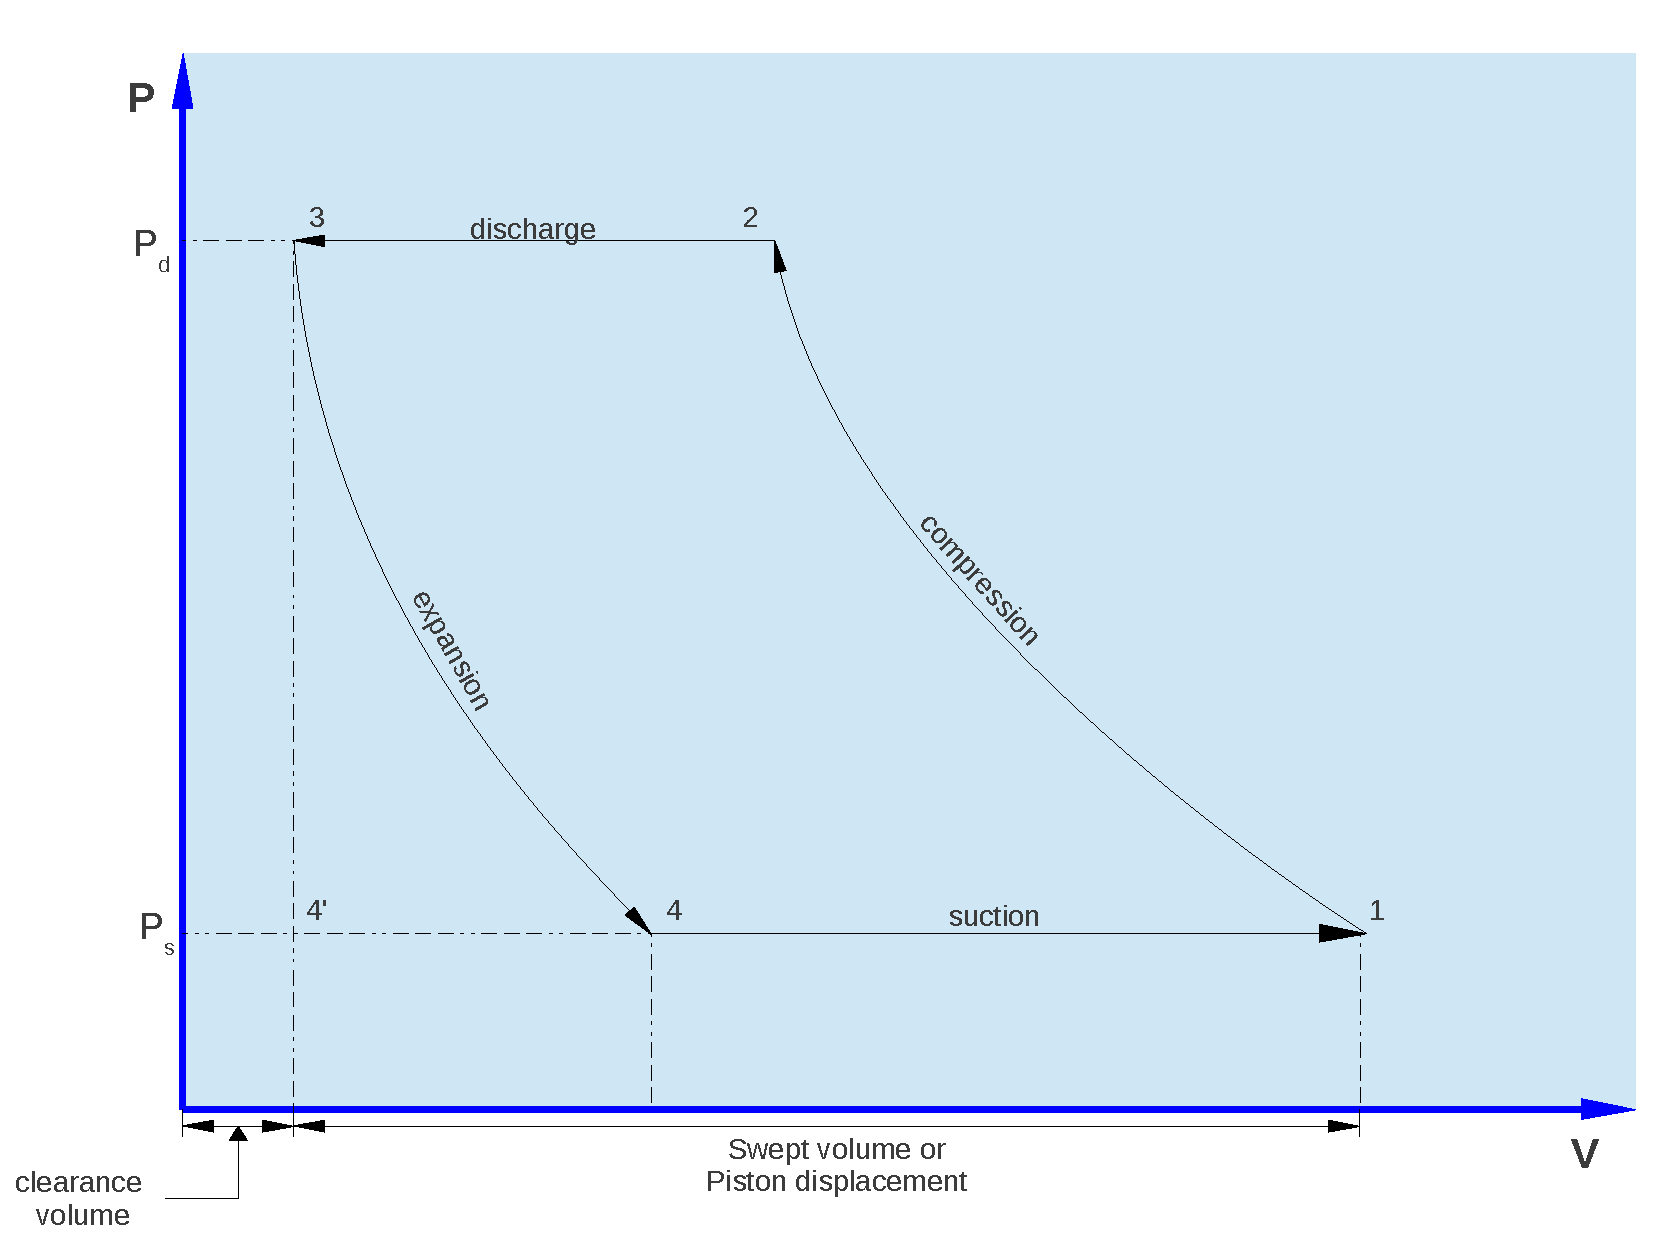
\includegraphics[width=12.cm,height=8.cm,clip]{./Pics/Overview_Refrig29}
  \end{center}
  \caption{Strokes in the compressor: Problem \ref{Ex4}.}\label{ex4_pic}
\end{figure}  


%%%
%%% Rajput (pg 739-40)
%%%
\item \label{Ex4} {\it Derive the clearance volumetric efficiency $\left(\eta_{cv}\right)$ expression in a compressor (Fig. \ref{ex4_pic}) assuming polytropic expansion.}
During the compression stage (Fig. \ref{ex4_pic}) in the refrigeration cycle, the motion of the piston within the cylinder can be described by the four strokes:
\begin{itemize}
\item (4-1): suction;
\item (1-2): compression;
\item (2-3): discharge;
\item (3-4): expansion;
\item (4-1): suction.
\end{itemize}
During the suction stroke (4-1), the vapour contained in the clearance space of the cylinder at the discharge pressure, $P_{d}$, expands (3-4). The suction valve is opened when the pressure drops to the suction pressure -- $P_{s}$, and the volume sucked is $\left(V_{1}-V_{4}\right)$ whereas the swept volume is $\left(V_{1}-V_{4}'\right)$.  The clearance volumetric efficiency is formally defined as,
\begin{equation}
\eta_{cv}=\frc{V_{1}-V_{4}}{V_{1}-V_{4'}}=\frc{V_{1}-V_{4}}{V_{1}-V_{3}} 
\label{clearancevolumetricefficiency}
\end{equation}
In a polytropic expansion process (3-4),
\begin{eqnarray}
 P_{3}V_{3}^{n} = P_{4}V_{4}^{n} &\Longrightarrow& P_{d}V_{3}^{n}=P_{s}V_{4}^{n} \nonumber \\
&& V_{4}=V_{3}\left(\frc{P_{d}}{P_{s}}\right)^{1/n} \label{polytropic}
\end{eqnarray}
We define the clearance ratio as
\begin{displaymath}
\mathcal{C}=\frc{\text{Clearance Volume}}{\text{Swept Volume}} = \frc{V_{3}}{V_{1}-V_{3}}
\end{displaymath}

Rearranging Eqn. \ref{clearancevolumetricefficiency},
\begin{eqnarray}
\eta_{cv} &=& \frc{V_{1}-V_{4}}{V_{1}-V_{3}} = \frc{\left(V_{1}-V_{4'}\right)-\left(V_{4}-V_{4'}\right)}{V_{1}-V_{3}} = \frc{\left(V_{1}-V_{3}\right)-\left(V_{4}-V_{3}\right)}{V_{1}-V_{3}} \nonumber \\
         &=& 1 - \frc{V_{4}-V_{3}}{V_{1}-V_{3}} \nonumber
\end{eqnarray}
Now substituting $V_{4}$ from Eqn. \ref{polytropic},
\begin{eqnarray}
\textcolor{blue}{\eta_{cv}} &=& 1 - \frc{V_{3}\left(\frc{P_{d}}{P_{s}}\right)^{1/n}-V_{3}}{V_{1}-V_{3}}=1+\frc{V_{3}}{V_{1}-V_{3}}\left[1-\left(\frc{P_{d}}{P_{s}}\right)^{1/n}\right] \nonumber \\
         &=& \textcolor{blue}{1 + \mathcal{C}\left[1-\left(\frc{P_{d}}{P_{s}}\right)^{1/n}\right]}
\end{eqnarray}

%%%
%%% Ameen (example 3.3, pg 50)
%%%
\item \label{Ex5} {\it An ice plant operates on the ideal vapour-compression cycle with superheated state using refrigerant fluid R134a.  The refrigerant enters the compressor as saturated vapour at 0.15 MPa and leaves the condenser as saturated liquid at 0.7 MPa.  Water enters the refrigerator cavity at 30$^{\text{o}}$C and leaves as ice at -5$^{\text{o}}$C. For an ice production rate of 10 kg per hour, determine the power input to the ice plant and the COP of the cycle. Also, sketch the $PH$ and $TS$ diagrams. Specific heats of ice and water are 2.1 and 4.18 kJ/(kg.K), respectively, and the latent heat of fusion of ice is 334 kJ/kg. Repeat the same procedure for ammonia and propane as refrigerat fluid.}


%%%
%%% Ameen (example 3.9, pg 60)
%%%
\item \label{Ex6} {\it In an ammonia refrigeration system, the evaporator supplies 300kW of refrigeration at -30$^{\text{o}}$C.  The system uses 2-stage compression as shown in the Fig. \ref{fig:ex6}, with intercooling and removal of flash gas.  The condensing temperature is 35$^{\text{o}}$C.
    \begin{enumerate}
     \item Sketch the $PH$ diagram;
     \item Calculate the power required by the compressors;
     \item Determine the coefficient of performance.
    \end{enumerate}

Assume that the intermediate pressure is expressed as: $P_{i}=\sqrt{P_{5}P_{1}}$.}
   \begin{figure}[h]
    \begin{center}
     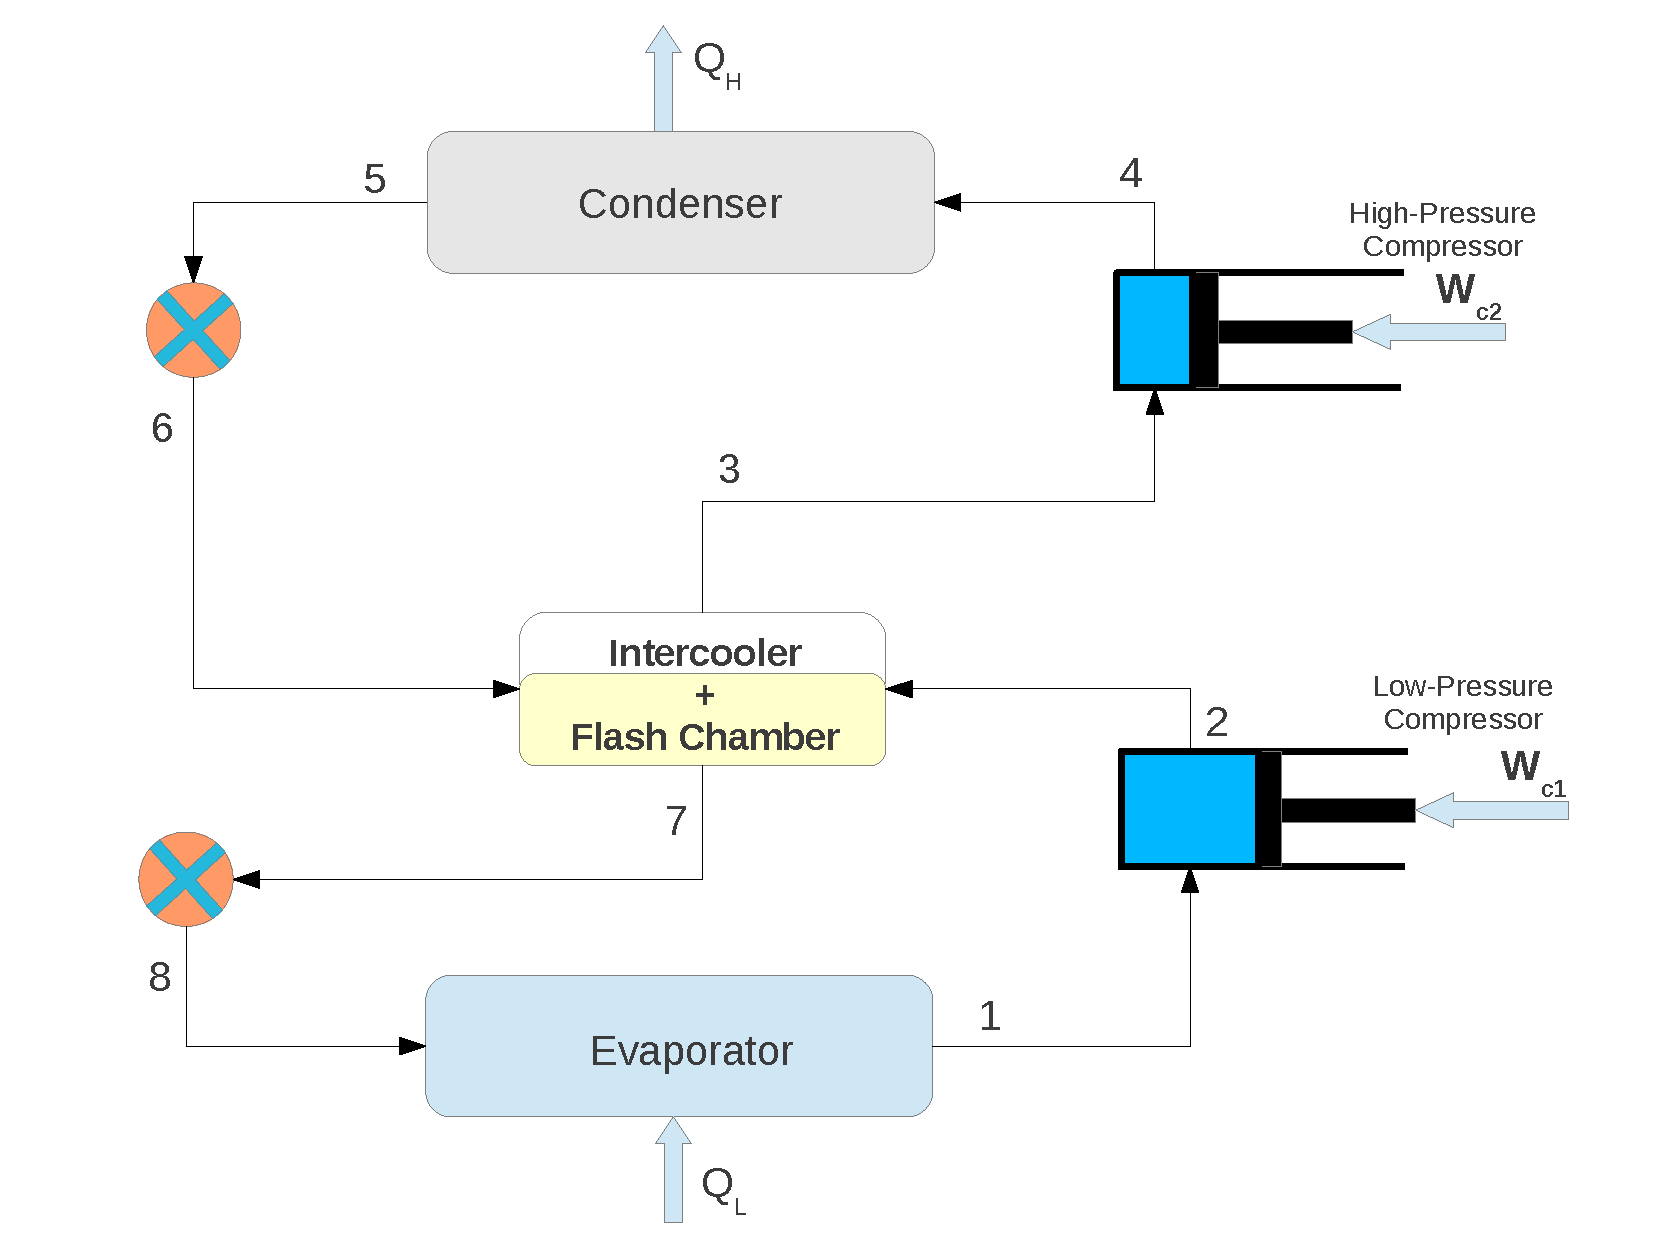
\includegraphics[width=10.cm,height=10.cm,clip]{./Pics/Overview_Refrig30}
    \end{center}
     \caption{Two-stage vapour-compression cycle: Problems \ref{Ex6} and \ref{Ex9}.} \label{fig:ex6} 
  \end{figure}  


%%%
%%% Saphiro 10.15
%%%
\item \label{Ex7} {\it A vapour-compression refrigeration cycle operates with Refrigerant R-134a as refrigerant fluid. Saturated vapour enters the compressor at 2 bar, and saturated liquid exits the condenser at 8 bar. The isentropic compressor efficiency is of 80$\%$. The mass flow rate  of refrigerant is 7 kg/min. Determine:
\begin{enumerate}
\item Compressor power;
\item Refrigerant effect (in tons and in kJ/s) and;
\item COP.
\end{enumerate}
}

%%%
%%% Saphiro 10.21
%%%
\item \label{Ex8} {\it In a vapour-compression refrigeration cycle operating with ammonia as refrigerant fluid, the refrigerating capacity is of 150 kW. Ammonia leaves the evaporator as saturated vapor at -22$^{\text{o}}$C and is driven to the condenser at 16 bar and 160$^{\text{o}}$C and leaves as saturated liquid at 16 bar. Assume that there is no relevant mechanical or thermal energy losses in and between the components of the cycle and also with the surroundings. Determine:
\begin{enumerate}
\item Mass flow rate of the refrigerant in kg/s;
\item Power input to the compressor in kW;
\item COP;
\item isentropic efficiency of the compressor.
\end{enumerate} 
}


%%%
%%% Saphiro 10.30
%%%
\item \label{Ex9} {\it An ammonia-based two-stage vapour-compression refrigeration system (Fig. \ref{fig:ex6}) uses a direct contact heat exchanger to achieve inter-cooling. The evaporator has a refrigerating capacity of 30 tons and produces -30$^{\text{o}}$C saturated vapour at its exit. In the first compressor stage, ammonia is compressed adiabatically to 5.5 bar, which is the pressure in the direct contact heat exchanger. Saturated vapour at 5.5 bar enters the second compressor stage and is compressed adiabatically to 18 bar.  Each compressor stage has an isentropic efficiency of 85$\%$. Assume that there are no mechanical or thermal energy losses within the cycle and to the surroundings. Saturated liquid enters each expansion valve. Determine:
\begin{enumerate}
\item The ratio of mass flow rates $\dot{m}_{3}/\dot{m}_{1}$;
\item Power input to each compressor stage $\left(W_{c,1},\;W_{c,2}\right)$;
\item COP.
\end{enumerate}
}


%%%
%%% Rajput Ex 14.24
%%%
\item \label{Ex10} {\it A heat pump operates in a vapour-compression cycle using Refrigerant-22 (R-22) as working fluid.  R-22 is compressed from saturated vapour at 2 bar to the condenser pressure of 12 bar.  The isentropic efficiency of the compressor is of 80$\%$. Saturated liquid enters the throttling valve at 12 bar. 80$\%$ of the heat rejected is transferred to the heated space which has a total heating requirement of 500 kJ/min. Determine:
\begin{enumerate}
\item (A)-(H) in the Table below:

%\begin{table}[h]
\begin{center}
\begin{tabular}{ || c || c | c | c | c || }
\hline\hline
        & {\bf Pressure}  &  {\bf Enthalpy}  & {\bf Entropy}     & {\bf State}  \\
        & {\bf (bar)}     &  {\bf (kJ/kg)}   &  {\bf (kJ/kg.K)}  &              \\
\hline\hline
{\bf 1} &   2.0           &       (A)        &      (B)          &  Saturated Vapour \\
{\bf 2} &   12.0          &       (C)        &      --           &  (D)          \\
{\bf 3} &   12.0          &       (E)        &      --           &  (F)        \\
{\bf 4} &   --            &       (G)        &      --           &  (H)       \\ 
\hline\hline
\end{tabular}
\end{center}
%\end{table}

\item Mass flow rate of the R-22 in kg/min.
\item Actual work in the compressor.
\item Coefficient of performance.

\end{enumerate}

}


%%%
%%% Rajput 14.19 modified
%%%
\item \label{Ex11} {\it A refrigerant fluid in a single-stage vapour-compression cycle produces a refrigerant capacity of 35 kW (thermodynamics properties in the table below). Saturated vapour leaves the evaporator at 1.50 bar and is compressed into superheated vapour at 9.0 bar. Determine
\begin{enumerate}
\item Mass flow rate of the refrigerant;
\item Power given to the compressor;
\item Piston displacement assuming that the expansion stroke follows $PV^{1.21}$ = constant. The volumetric efficiency of the piston is given by
\begin{displaymath}
\eta_{vol}=1 + \mathcal{C} - \mathcal{C} \left(\frac{P_{d}}{P_{s}}\right)^{n}
\end{displaymath}
where $\mathcal{C}$ is the clearance ratio, $P_{d}$ and $P_{s}$ are the discharge and suction pressures, respectively. The compressor operates at 150 rpm and has a clearance volume of 1.5$\%$ of the stroke volume.
\item Sketch the $TS$ diagram of the refrigeration process and the $PV$ diagram of the strokes in the compressor.
\end{enumerate}
Assume that the heat capacity of the fluid is $C_{p}=4.818$ kJ/(kg.K).
\begin{center}
\begin{tabular}{|c c| c c c c c | }
\hline
$P$             & $T_{s}$  & $V_{g}$  & $H_{f}$  & $H_{g}$   &  $S_{f}$   &  $S_{g}$    \\
(bar)   &  ($^{\text{o}}$C)  & $\left(\text{m}^{3}/\text{kg}\right)$ & (kJ/kg) & (kJ/kg) & (kJ/(kg.K)) &  (kJ/(kg.K))  \\
\hline
1.50  &  -25.22  & 0.7787 & 65.32 & 1410.61 & 0.2712 & 5.6973  \\
9.00  &   21.52  & --     & 281.53 & 1460.97 & 1.0649 & 5.0675  \\
\hline
\end{tabular}
\end{center}
}

%%%
%%% Shapiro 10.31
%%%
\item \label{Ex12} {\it Ammonia is used as a refrigerant fluid in a 2-stage vapour-compression refrigeration system (Fig. \ref{Ex12:Fig}) with 2 evaporators and a heat exchanger. Saturated vapour from the evaporator 1 enters the compressor 1 at 1.2 bar and exits at 5 bar. Evaporator 2 operates at 5 bar with saturated vapour exiting towards the heat exchanger. The condenser pressure is 14 bar and saturated liquid exits the condenser. Each compressor stage has an isentropic efficiency of 80$\%$. The refrigeration capacity of evaporators 1 and 2 are of 5 and 10 tons, respectively. 
\begin{enumerate}
 \item Determine the temperature of the ammonia at the exit of each evaporator.
 \item Calculate the power input to each compressor and the overall coefficient of performance of the cycle.
 \item Sketch the TS diagram of the cycle.
\end{enumerate}

}

\begin{figure}[h]
\begin{center}
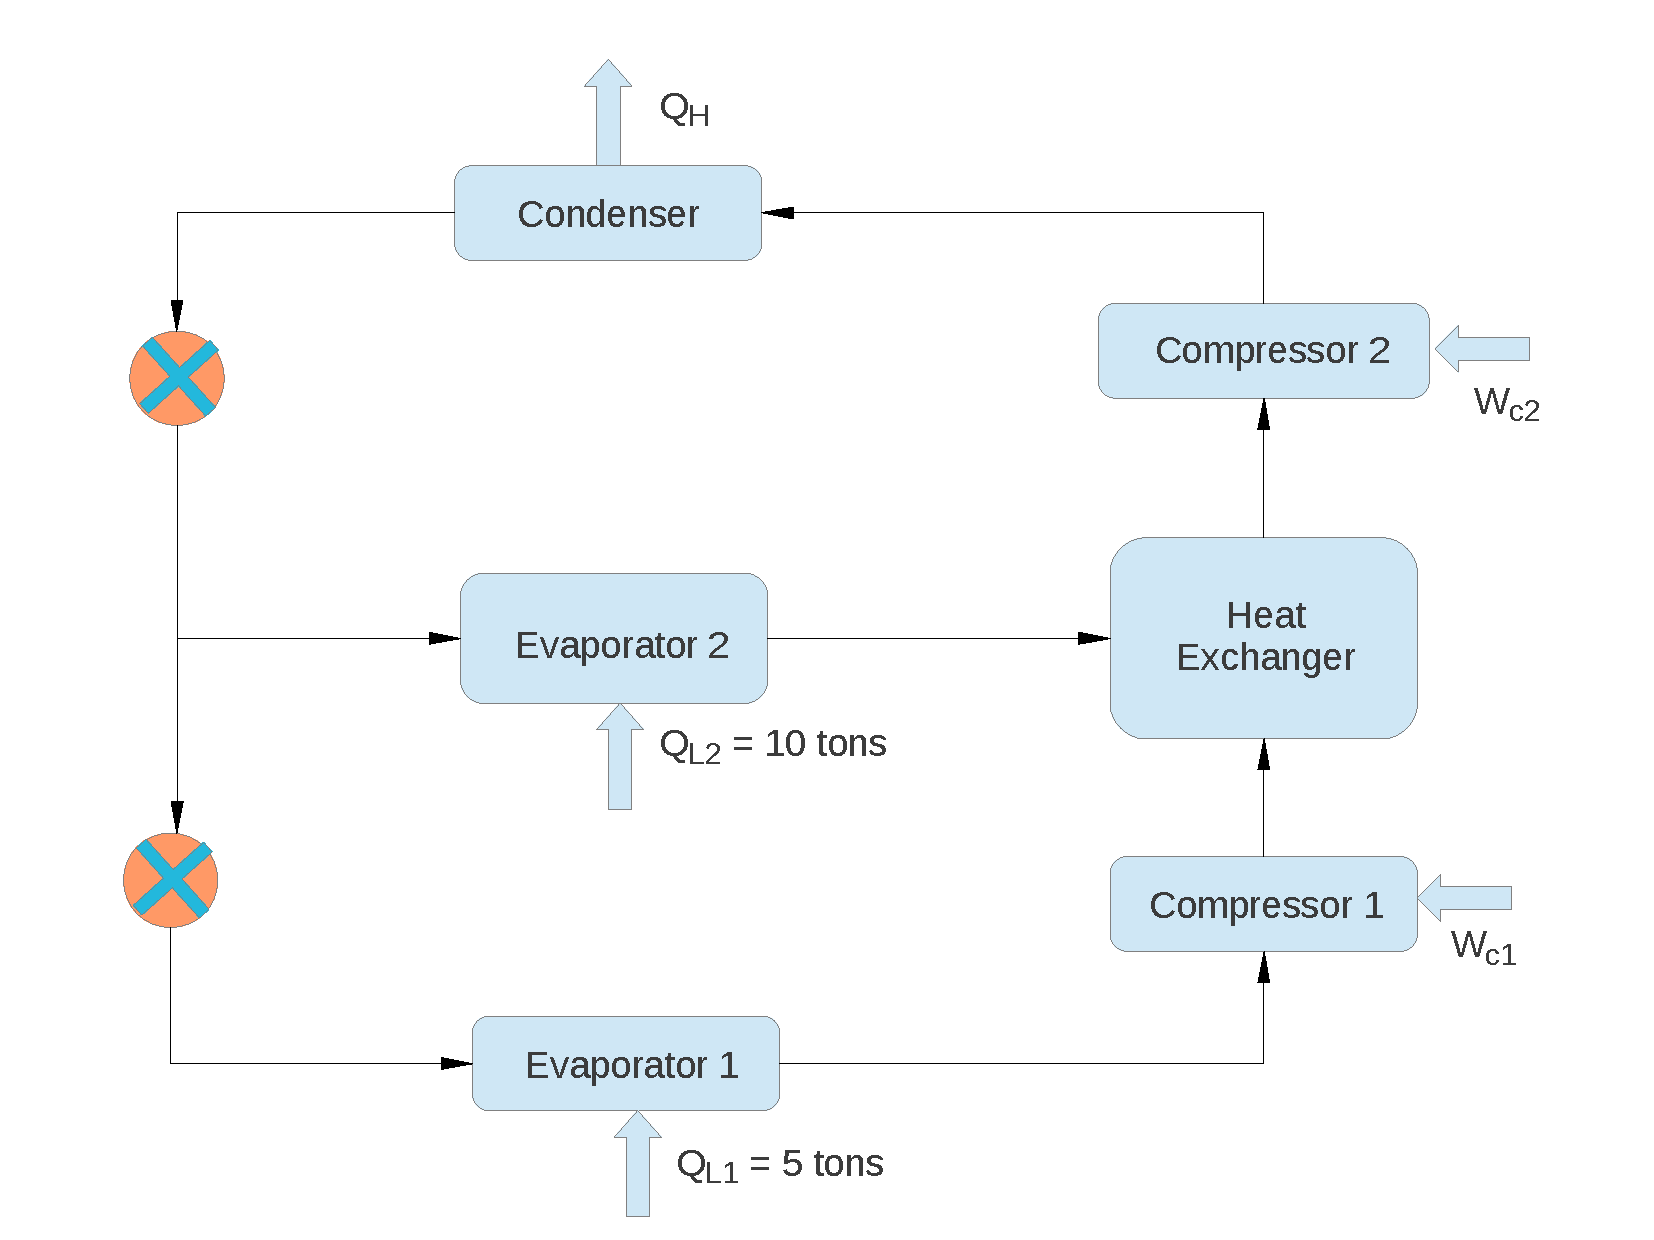
\includegraphics[width=16.0cm,height=12.0cm]{./Pics/Overview_Refrig41}
\end{center}
\caption{Two-stage vapour-compression refrigeration cycle: Problem \ref{Ex12}.}\label{Ex12:Fig}
\end{figure}




%%%
%%% Shapiro 10.42
%%%
\item \label{Ex13} {\it R-22 is the refrigerant fluid in a geothermal heat pump system for a house (Fig. \ref{Ex13:Fig}). The heat pump uses underground water from a well $\left(T_{\text{w}}^{\text{in}}=13^{\text{o}}\text{C}; T_{\text{w}}^{\text{out}}=7^{\text{o}}\text{C}\right)$ to produce a heating capacity of 4.2 tons. Determine:
\begin{enumerate}
 \item Volumetric flow rate of heated air to the house $\left(m^{3}/s\right)$;
 \item Isentropic efficiency $\left(\eta_{c}\right)$ and power $\left(\dot{W}_{c}\right)$ of the compressor;
 \item Coefficient of Performance;
 \item Volumetric flow rate of water from the geothermal well $\left(l/h\right)$;
 \item Sketch the $TS$ diagram.
\end{enumerate}
Given the heat capacity $\left(C_{p}^{\text{air}}=1.004\displaystyle\frac{kJ}{kg.K}\right)$ and molecular weight $\left(MW^{\text{air}}=28.97\displaystyle\frac{kg}{kgmol}\right)$ of air and heat capacity of water $\left(C_{p}^{\text{water}}=4.1813\displaystyle\frac{kJ}{kg.K}\right)$.
}

\begin{figure}[h]
\begin{center}
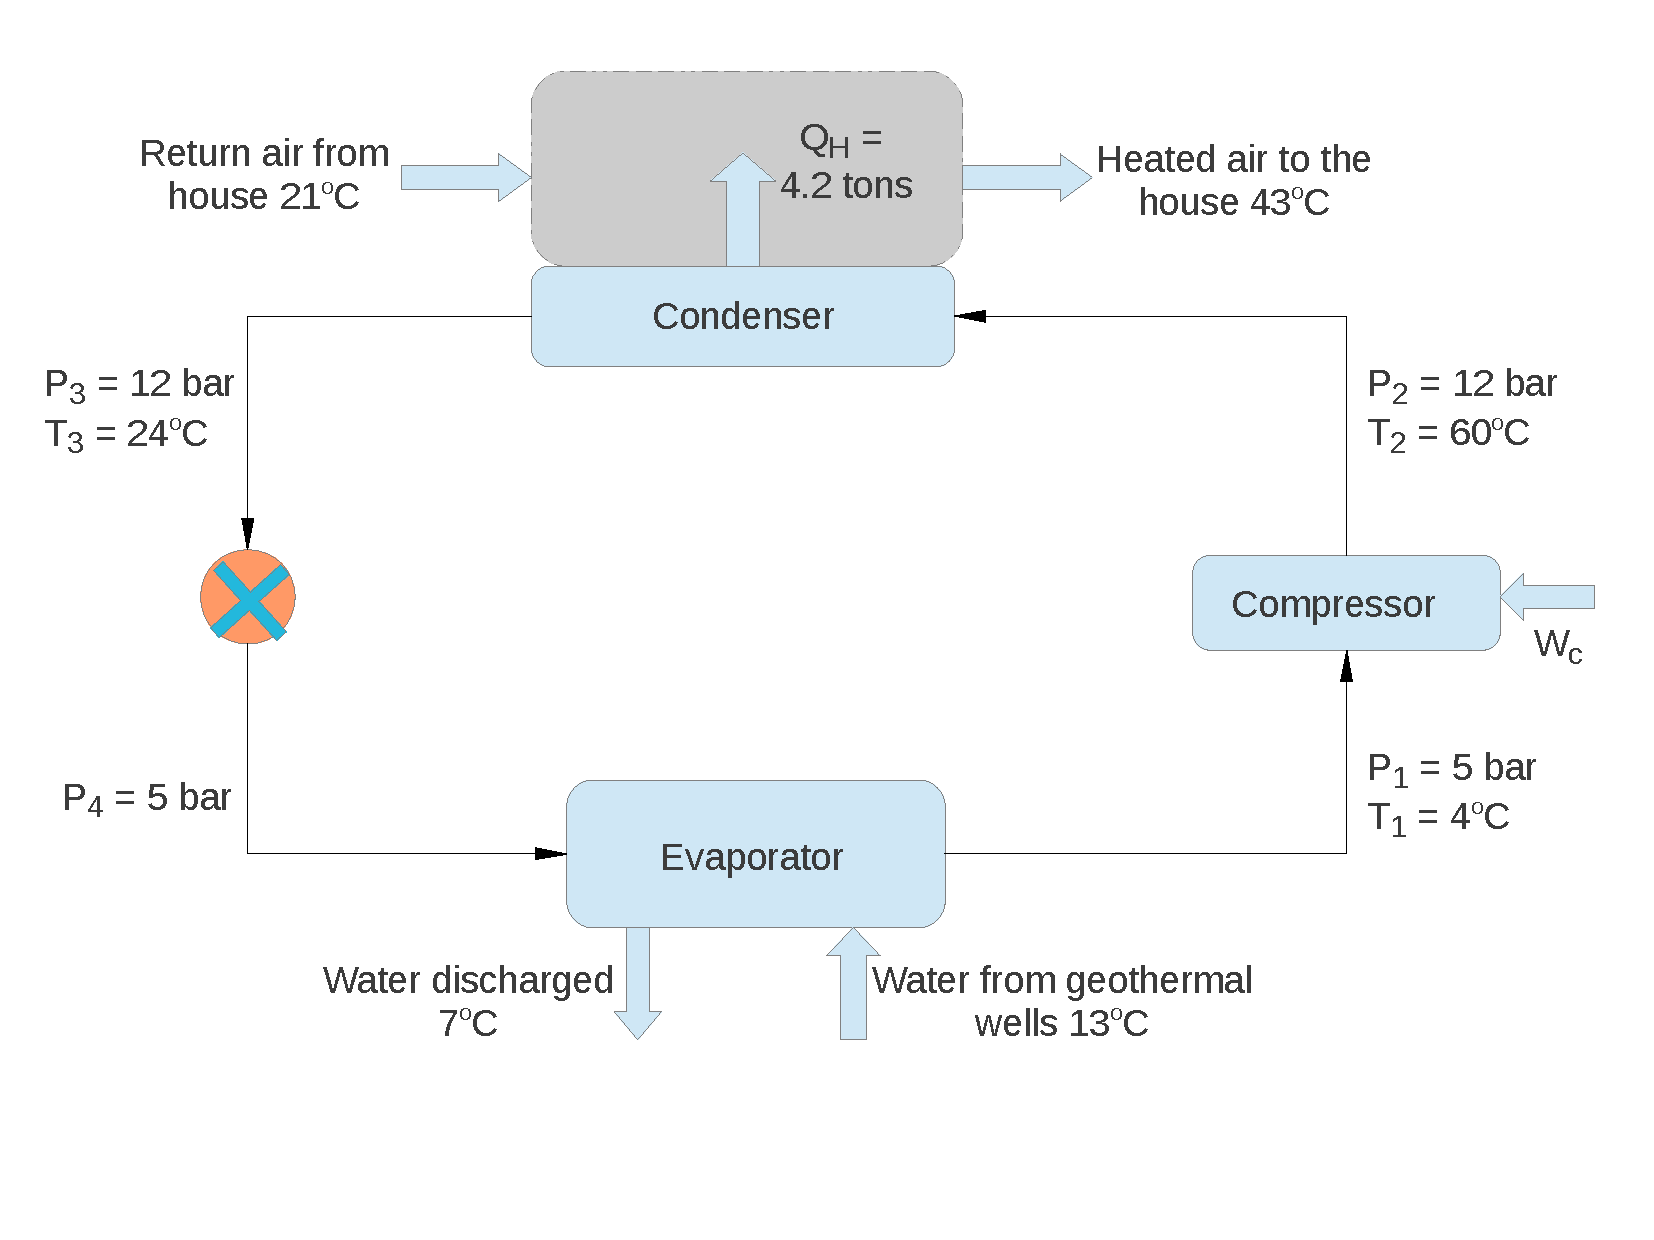
\includegraphics[width=16.0cm,height=12.0cm]{./Pics/Overview_Refrig42}
\end{center}
\caption{Heat pump cycle: Problem \ref{Ex13}.}\label{Ex13:Fig}
\end{figure}


\pagebreak

%%%
%%% Jeff
%%%
\item \label{Ex14} {\it A Thermal engineer is hired to design coupled steam-power and refrigeration plants (Fig. \ref{Ex14:Fig}). The thermal plant (I) operates 100 kg/h steam in 3-turbines reheat Rankine cycle with initial conditions and efficiencies described in Tables \ref{Ex14:Tab1} and \ref{Ex14:Tab2}. 0.1$\%$ of the power generated by the set of turbines in {\bf I} is used in the compressor of the refrigeration unit {\bf II}. The refrigeration system operates with a proprietary working fluid, $\mathcal{X}$ with thermodynamic properties as described in Table \ref{Ex14:Tab3}. Determine:
\begin{enumerate}
\item Net work for the thermal cycle {\bf I} $\left(\displaystyle\frac{\dot{W}_{\text{cycle}}}{\dot{m}_{\text{water}}}\right)$ and the power produced by the set of turbines $\left(\dot{W}_{c}\right)$;
\item Extensive properties of units {\bf I} and {\bf II} in Table \ref{Ex14:Tab1} -- {\bf A}-{\bf V} and {\bf i}-{\bf xii};
\item Mass flow rate of refrigerant fluid $\mathcal{X}$ and refrigerating capacity;
\item Piston displacement assuming that the expansion stroke follows $PV^{1.3}$ = constant. The volumetric efficiency of the piston is given by
\begin{displaymath}
\eta_{vol}=1 + \mathcal{C} - \mathcal{C} \left(\frac{P_{d}}{P_{s}}\right)^{n}
\end{displaymath}
where $\mathcal{C}$ is the clearance ratio, $P_{d}$ and $P_{s}$ are the discharge and suction pressures, respectively. The compressor operates at 360 rpm and has a clearance volume of 4$\%$ of the stroke volume.
\end{enumerate}

}

\begin{figure}[h]
\begin{center}
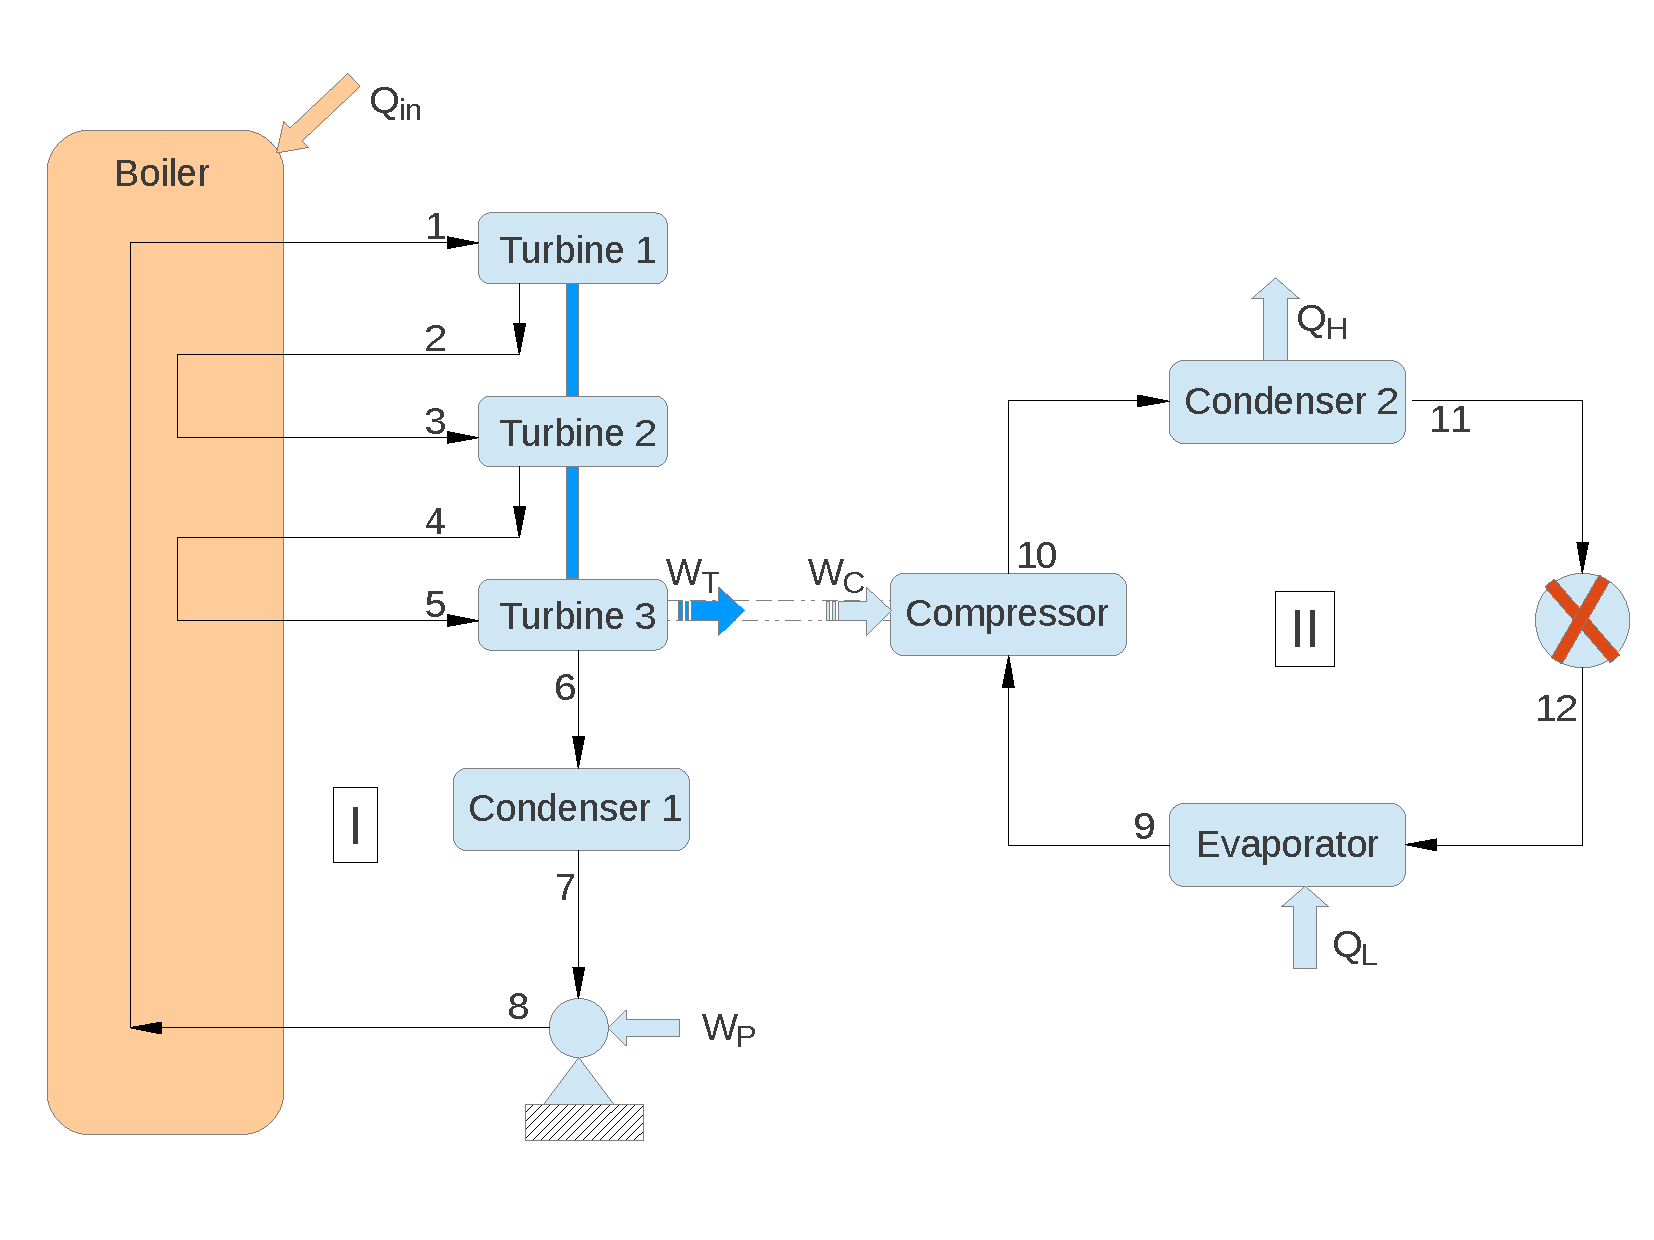
\includegraphics[width=16.0cm,height=12.0cm]{./Pics/Overview_Refrig43}
\end{center}
\caption{Coupled reheat Rankine steam and reversed-Rankine refrigeration units --  Problem \ref{Ex14}.}\label{Ex14:Fig}
\end{figure}

\begin{table}[h]
\begin{center}
\begin{tabular}{ || c || c | c | c | c | c || c ||}
\hline\hline
{\bf Flow}& {\bf Pressure}  &  {\bf Temperature}   &  {\bf Enthalpy}  & {\bf Entropy}     & {\bf State}  & {\bf Quality of} \\
          & {\bf (bar)}     & {\bf ($^{\text{o}}$C)} &  {\bf (kJ/kg)}   &  {\bf (kJ/kg.K)}  &              & {\bf steam}      \\
\hline\hline
{\bf 1}   &   200.0         &      600         &      (A)          &      (B)             & (C)          &  --              \\
{\bf 2}   &   5.0           &       --         &      (D)          &      --              & --           &  (E)             \\
{\bf 3}   &   5.0           &      240         &      (F)          &      (G)             & (H)          &  --              \\
{\bf 4}   &   1.0           &      --          &      (I)          &      --              & --           &  (J)             \\ 
{\bf 5}   &   1.0           &    99.63         &      (K)          &     (L)              &  (M)         &   --             \\ 
{\bf 6}   &   0.23          &      --          &      (N)          &     --               &  --          &  (O)             \\
{\bf 7}   &   (P)           &      --          &      (Q)          &      (R)             &  (S)         &   --             \\              
{\bf 8}   &   (T)           &      --          &      (U)          &       --             & (V)          & --               \\
\hline \hline
{\bf 9}   &   2.0           &      --          &      (i)          &      (ii)            &  (iii)       &  --              \\
{\bf 10}  &  16.0           &     (iv)         &      (v)          &      (vi)            &   (vii)      &   --             \\ 
{\bf 11}  &  (viii)         &     --           &      (ix)         &      --              &  (x)         &   --             \\
{\bf 12}  &   (xi)          &    --            &     (xii)         &      --              &   --         &    --            \\ 
\hline\hline
\end{tabular}
\end{center}
\caption{Information on the steam-power and refrigeration cycles (Problem \ref{Ex14}).}\label{Ex14:Tab1}
\end{table}

\begin{table}[h]
\begin{center}
\begin{tabular}{||c | c c c c | c||}
\hline\hline
               &  {\bf Turbine 1} & {\bf Turbine 2}  & {\bf Turbine 3}  & {\bf Pump}  & {\bf Compressor}\\
{\bf Efficiency}&    0.88          &   0.85           &     0.85         &  0.92      &  1.00           \\
\hline\hline
\end{tabular}
\end{center}
\caption{Efficiencies of the equipment used in the coupled units (Problem \ref{Ex14}).}\label{Ex14:Tab2}
\end{table}


\begin{table}[h]
\begin{center}
\begin{tabular}{|c c| c c c c c c | }
\hline
$P$             & $T_{s}$   & $V_{f}\times 10^{-3}$  &  $V_{g}$   & $H_{f}$  & $H_{g}$   &  $S_{f}$   &  $S_{g}$    \\
(bar)   &  ($^{\text{o}}$C)  & $\left(\text{m}^{3}/\text{kg}\right)$ & $\left(\text{m}^{3}/\text{kg}\right)$ & (kJ/kg) & (kJ/kg) & (kJ/(kg.K)) &  (kJ/(kg.K))  \\
\hline
2.00    &  -18.86  & 1.5071  &  0.5946   &   93.80  & 1419.31  &  0.3843  & 5.5969   \\
16.00   &   41.03  & 1.7306  &  0.0808   &  376.46  &  1470.23 &  1.3729  & 4.8542   \\
\hline
\end{tabular}
\end{center}
\caption{Thermodynamic properties of refrigerant fluid $\mathcal{X}$ (Problem \ref{Ex14}).}\label{Ex14:Tab3}
\end{table}



\end{enumerate}
%\pagebreak
%%%
%\subsection{XXX}

%\end{Large}
%
\pagebreak

\subsection{Carnot and Rankine Steam Cycles}


\begin{enumerate}

%%%
%%%
%%%
\item {\it In a turbine, steam at 20 bar, 360$^{o}$C is expanded to 0.08 bar. The steam is condensed into saturated liquid water. The pump feeds the water back into the boiler. Assume ideal processes, calculate the net work per kg of steam and the cycle efficiency.}\label{Example_01_01}

\begin{figure}[h]
\begin{center}
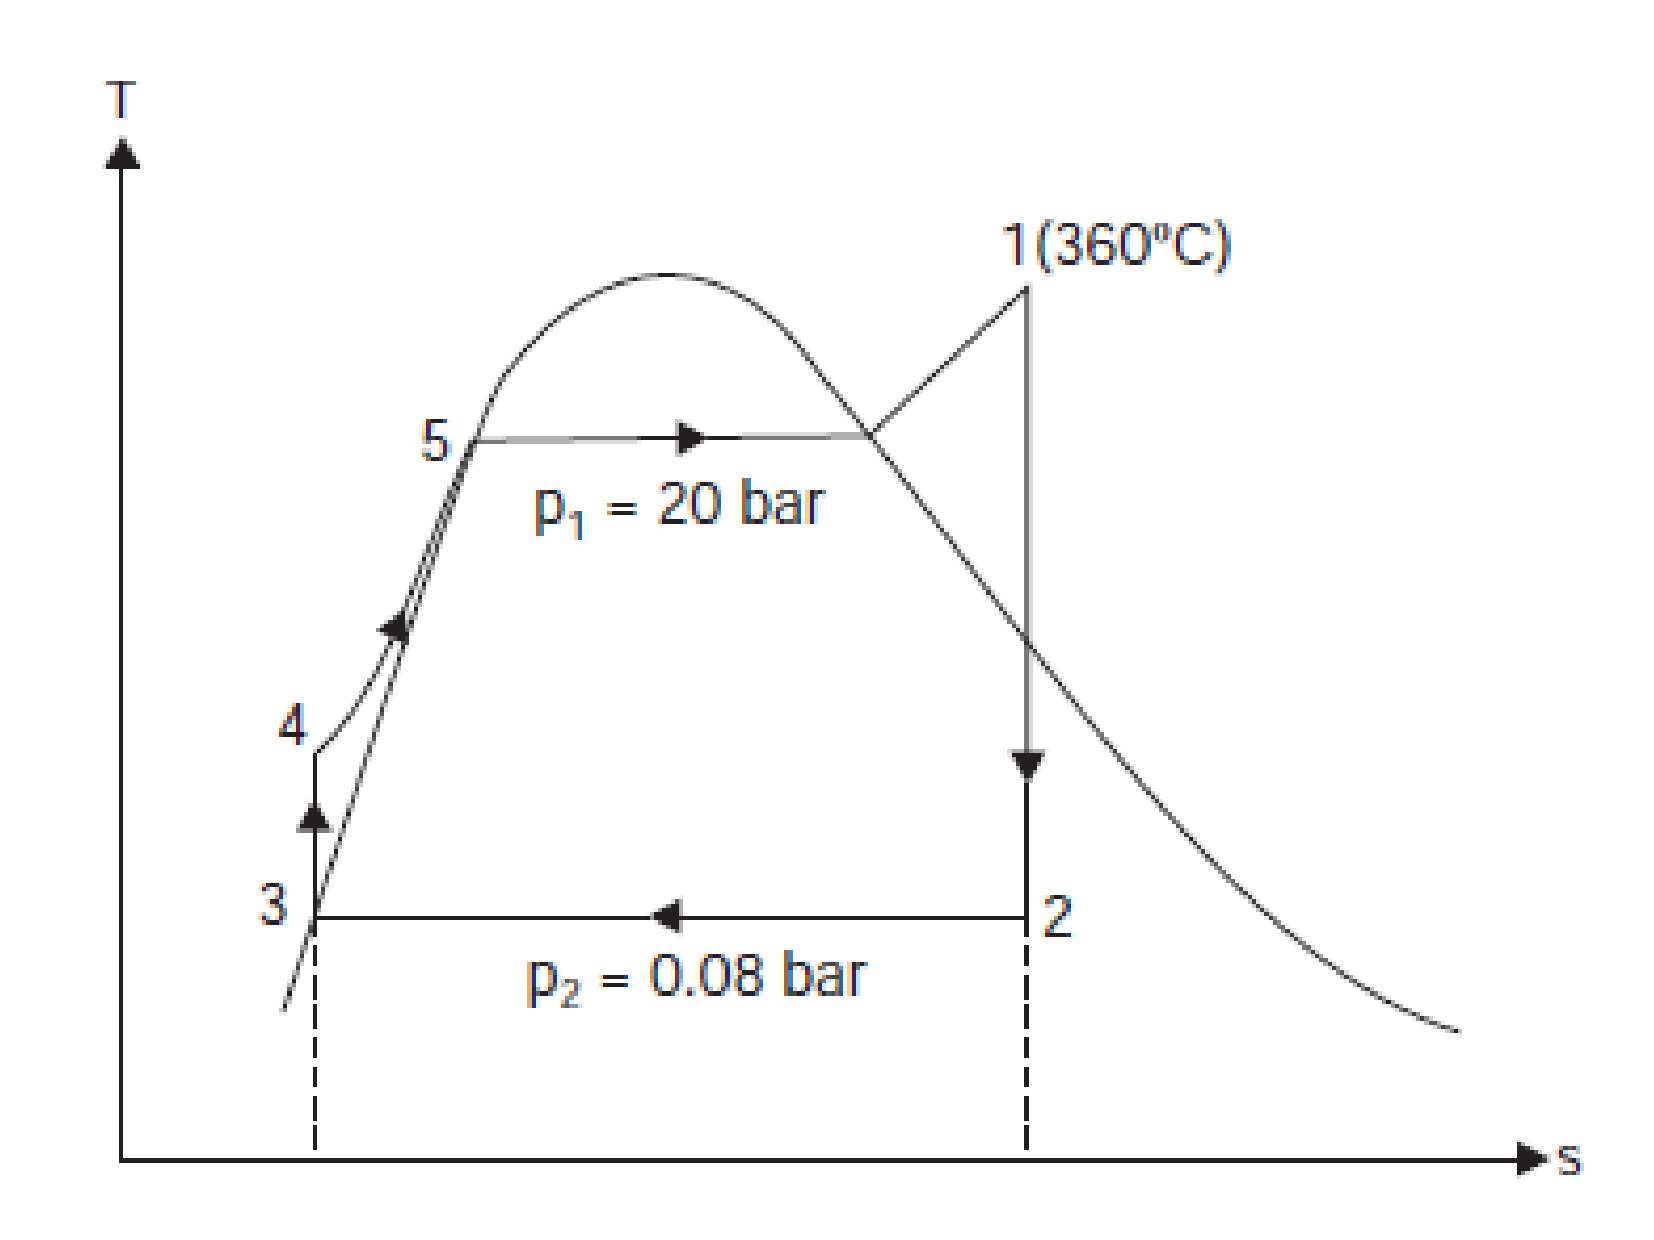
\includegraphics[width=13.0cm,height=8.0cm]{./../../ThermalEngines/Pics/example01_01}
\end{center}
\caption{Carnot and Rankine Cycles: Ts diagram -- Example \ref{Example_01_01}.}
\label{Example01_01:Pic1}
\end{figure}

As the process {\it 1-2} is isentropic (Fig. \ref{Example01_01:Pic1}), $s_{1}=s_{2}$ and using the data in Table \ref{Example01_01:Table1},
\begin{eqnarray}
&& 6.9917 = s_{f,2}+x_{2}s_{fg,2} = 0.5926 + 7.6361 x_{2} \;\; \Longrightarrow \;\; x_{2}= 0.838 \nonumber \\
&& h_{2} = h_{f,2}+ x_{2}h_{fg,2} \;\; \Longrightarrow h_{2}=2187.68\;kJ/kg \nonumber
\end{eqnarray}

\begin{center}
\begin{table}[h]
\begin{tabular}{c c c c c c c c c }
\hline
                    & $P$   & $T$ &  $h_{f}$  & $h_{fg}$ & $s_{f}$      & $s_{fg}$      & $s_{g}$        &   $v_{f}$ \\
                    & (bar) & (K) &  (kJ/kg) &  (kJ/kg) & (kJ/(kg.K)) & (kJ/(kg.K))   & (kJ/(kg.K))   &$\left(m^{3}/kg\right)$ \\
\hline
{\it Boiler}        & 20    & 633.15& 3159.3  & --      & 6.9917      & --            & --             & --  \\
\hline
{\it Condenser}     & 0.08  &  --  & 173.88  & 2403.1   & 0.5926      &  7.6361       & 8.2287         & 1.008$\times$10$^{-3}$ \\
\hline
\end{tabular}
\caption{Carnot and Rankine Cycles: Steam tables -- Example \ref{Example_01_01}.}
\label{Example01_01:Table1}
\end{table}
\end{center}

The net work $\left(W_{\text{net}}\right)$ is calculated from, $W_{\text{net}}=W_{\text{turbine}}-W_{\text{pump}}$. The work required by the pump is
\begin{eqnarray}
&& W_{\text{pump}}=h_{f,4}-h_{f,3}=v_{f,2}\left(P_{1}-P_{2}\right) = 1.008\times 10^{-3} \left[\frc{m^{3}}{kg}\right] \times (20-0.08) [bar] \times \left[\frc{100\;kJ/kg}{m^{3}.bar/kg}\right] = 2.008\; kJ/kg \nonumber \\
&& h_{f,4} = 2.008+h_{f,2}=175.89\;kJ/kg\nonumber
\end{eqnarray}
And the work produced by the tubine is defined as
\begin{displaymath}
W_{\text{turbine}}=h_{1}-h_{2} = 3159.3-2187.68= 971.62 \; kJ/kg
\end{displaymath}

And the net work is
\begin{eqnarray}
&& W_{\text{net}}=W_{\text{turbine}}-W_{\text{pump}} = 971.62-2.008 \nonumber \\
&& \textcolor{red}{W_{\text{net}}=969.61\frc{kJ}{kg}} \nonumber
\end{eqnarray}

The efficiency of the cycle is obtained by the relationship $\eta_{\text{cycle}}=\frc{W_{\text{net}}}{Q_{1}}$. The heat added into the boiler $\left(Q_{1}\right)$ is given by,
\begin{displaymath}
Q_{1}=h_{1}-h_{f,4}=3159.3-175.89=2983.41\;kJ/kg
\end{displaymath}
and the efficiency is
\begin{displaymath}
\textcolor{red}{\eta_{\text{cycle}}=\frc{969.61}{2983.41}=0.325\text{ or } 32.5\%}
\end{displaymath}


%%%
%%%
%%%
\item {\it A Rankine cycle operates between pressures of 80 and 0.1 bar and the maximum temperature is 873.15 K. Assuming that the steam turbine and condensate pump efficiencies are 90$\%$ and 80$\%$, respectively, calculate the specific work and thermal efficiency.}\label{Example_01_02}

From the saturated water and steam tables:

\begin{center}
\begin{table}[h]
\begin{tabular}{||c|c|c c|c c c|c c c||} 
\hline\hline
{\bf P (bar)} & {\bf T (K)} & \multicolumn{2}{|c|}{{\bf Specific Volume $\left(m^{3}/kg\right)$}} & \multicolumn{3}{|c|}{{\bf Specific Enthalpy (kJ/kg)}} & \multicolumn{3}{|c||}{{\bf Specific Entropy (kJ/(kg.K)}}  \\
\hline
              &             &  $v_{f}$                  &    $v_{g}$                              &  $h_{f}$    &  $h_{fg}$  &   $h_{g}$                 &  $s_{f}$  &  $s_{fg}$    &  $s_{g}$  \\
\hline\hline
0.1           & 318.99      &1.0103$\times$10$^{-3}$    & 0.1468$\times$10$^{2}$                  & 191.9   & 2392.3    & 2584.2              & 0.6488 & 7.5006  & 8.1494 \\
80            & 568.25      &1.385$\times$10$^{-3}$     & 0.0235                                  & 1317.0 & 1440.5   & 2757.5               & 3.2073 & 2.5351  & 5.7424  \\
\hline\hline
\end{tabular}
\caption{Carnot and Rankine Cycles: From Saturated water and steam tables.}
\label{Example01_01:Table2}
\end{table}
\end{center}


\begin{table}[h]
\begin{center}
\begin{tabular}{c c r}
\multicolumn{3}{c}{Superheated Steam} \\
\hline
\multirow{3}{*}{$P=80\;bar\;,\;T= 600^{o}C$} & $v$ & 0.486 m$^{3}$/kg \\
                           & $h$ & 3642 kJ/kg \\
                           & $s$ & 7.0206 kJ/(kg.K)\\
\hline
\end{tabular}
\end{center}
\caption{Carnot and Rankine Cycles: From Superheated Steam.}
\label{Example01_01:Table23}
\end{table}

Since $s_{1}=s_{2}$, the steam quality is calculated from,
\begin{eqnarray}
&& s_{2} = s_{f,2}+x_{2}s_{fg,2} \nonumber \\
&& 7.0206 =  0.6488 + 7.5006 x_{2} \nonumber \\
&& x_{2}= 0.85
\end{eqnarray}
and the enthalpy is obtained from 
\begin{displaymath}
h_{2}=h_{f,2}+x_{2}h_{fg,2} =191.9+0.85\times 2392.3 = 2225.36\; kJ/kg
\end{displaymath}
And the work


\begin{figure}[h]
\begin{center}
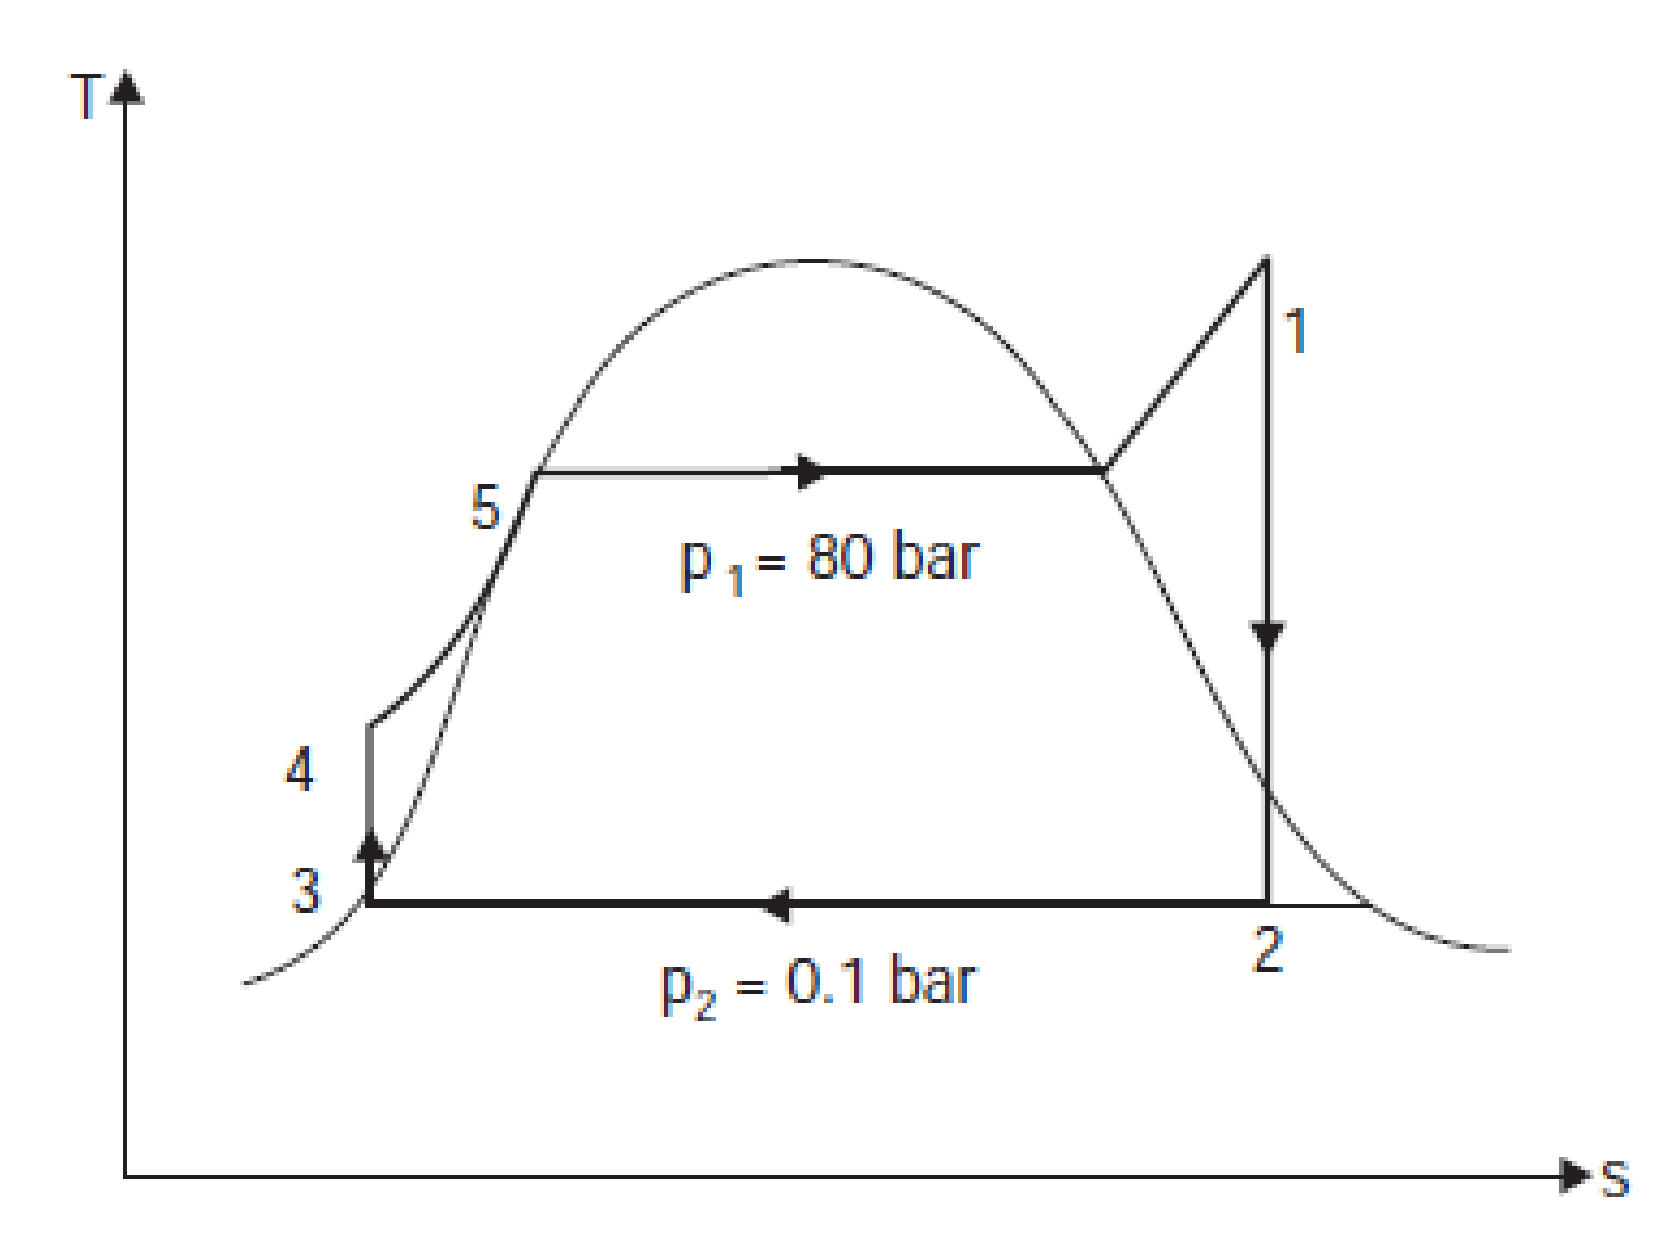
\includegraphics[width=13.0cm,height=8.0cm]{./../../ThermalEngines/Pics/example01_02}
\end{center}
\caption{Carnot and Rankine Cycles: Ts diagram -- Example \ref{Example_01_02}.}
\label{Example01_01:Pic2}
\end{figure}

%%%
%%%
%%%
\item {\it In a steam power plant operating on the Rankine cycle, steam enters the turbine at 30 bar and 623.15 K and later condensed at 0.1 bar. Calculate: (a) thermal efficiency; (b) thermal efficiency assuming that the steam is superheated to 873.15 K before entering the turbine; (c)thermal efficiency assuming that the boiler pressure is raised to 150 bar while the inlet temperature at turbine is maintained at  623.15 K.}\label{Example_01_03}


\begin{enumerate}
\item \label{example_01_03_a}The {\it Ts} diagrams of the cycle for all three cases can be seen in Fig. \ref{Example01_01:Pic3}, and the original phase states can assigned as 

\begin{tabular}{l l l l}
$P_{1}=0.1\;bar$ (saturated liquid) &  $P_{2}=30\;bar$ & $P_{3}=30\;bar$           & $P_{4}=0.1\;bar$ \\
$h_{1}=191.81\;kJ/kg$               &  $s_{2}=s_{1}$   & $T_{3}=623.15\;K$         & $s_{4}=s_{3}$ \\
$v_{1}=1.01\times 10^{-3}\;m^{3}/kg$ &                  & $h_{3}=3116.1\;kJ/kg$     &                 \\
                                    &                 & $s_{3}=6.7450\;kJ/(kg.K)$ &                 \\
\end{tabular}


\begin{figure}[h]
\begin{center}
\vbox{
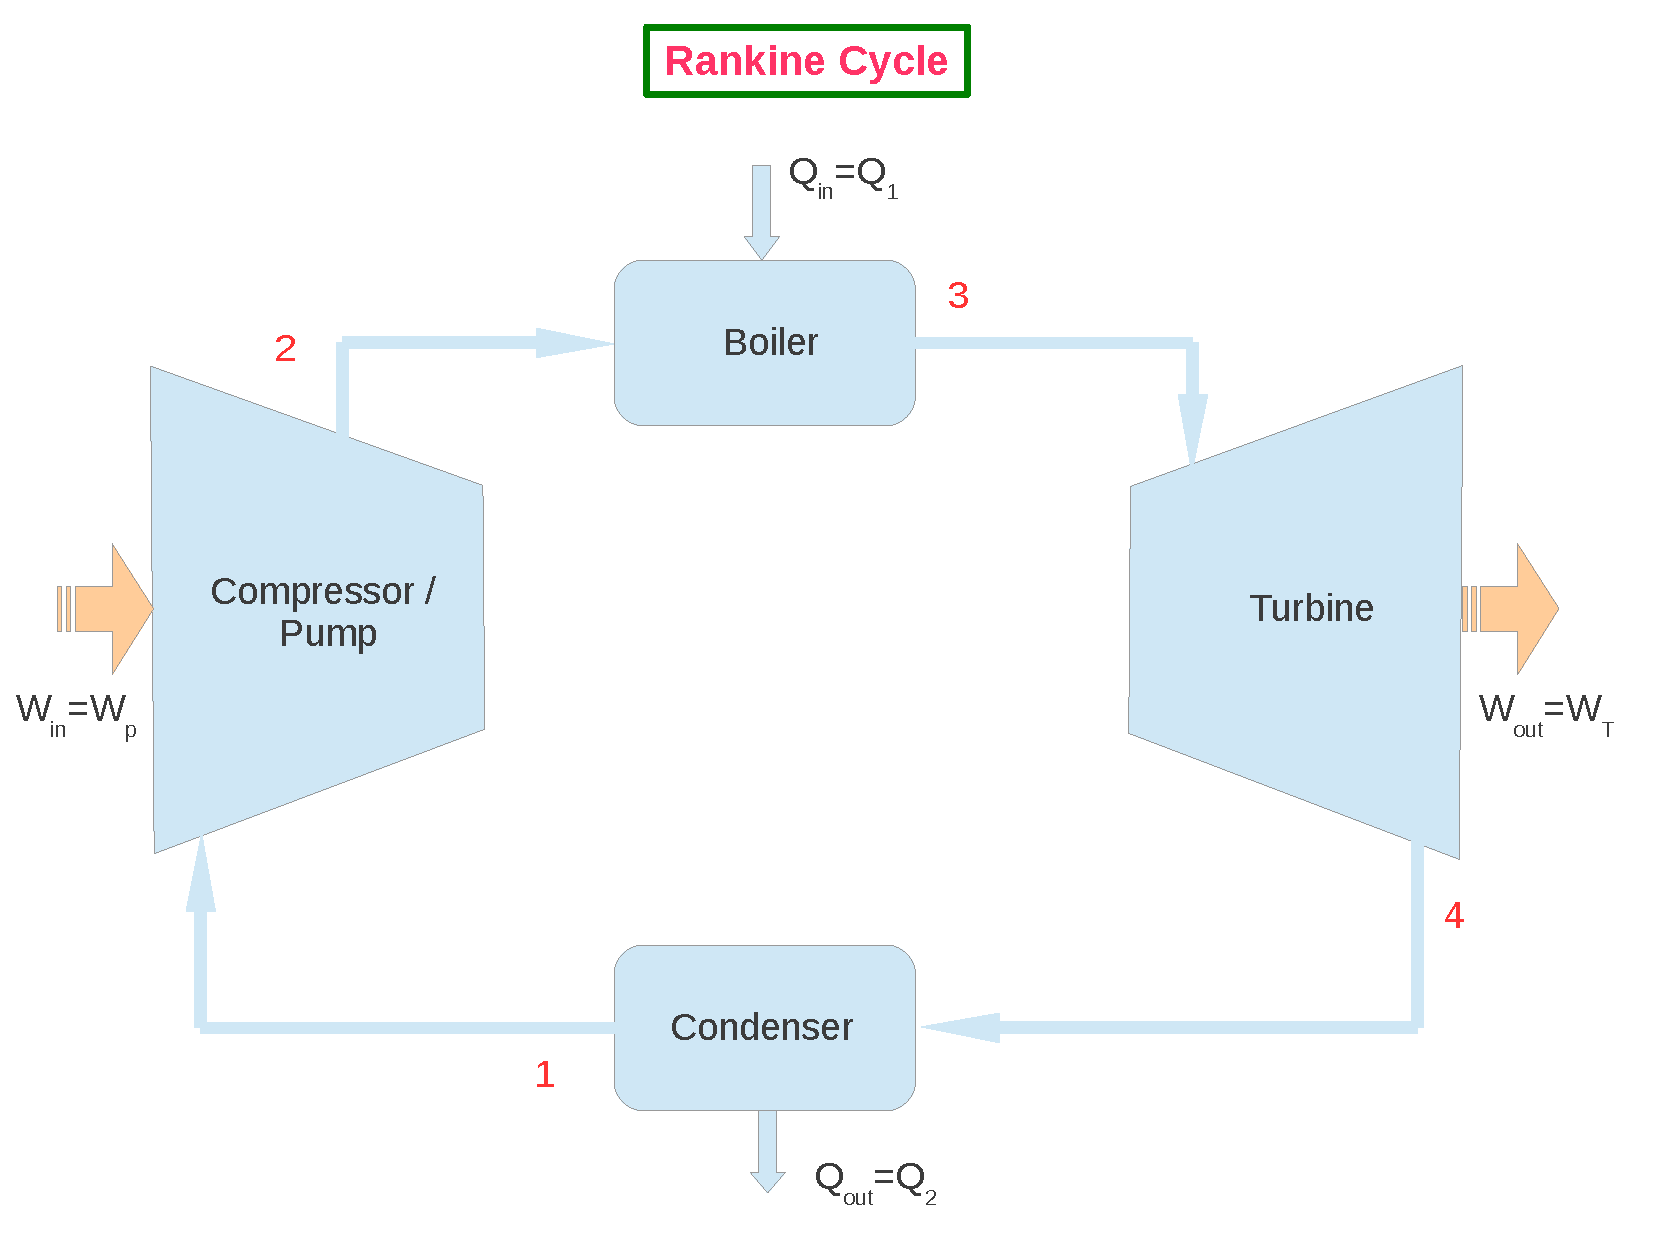
\includegraphics[width=13.0cm,height=9.0cm]{./../../ThermalEngines/Pics/Simple_Rankine_Cycle_2}
\vspace{-1.cm}
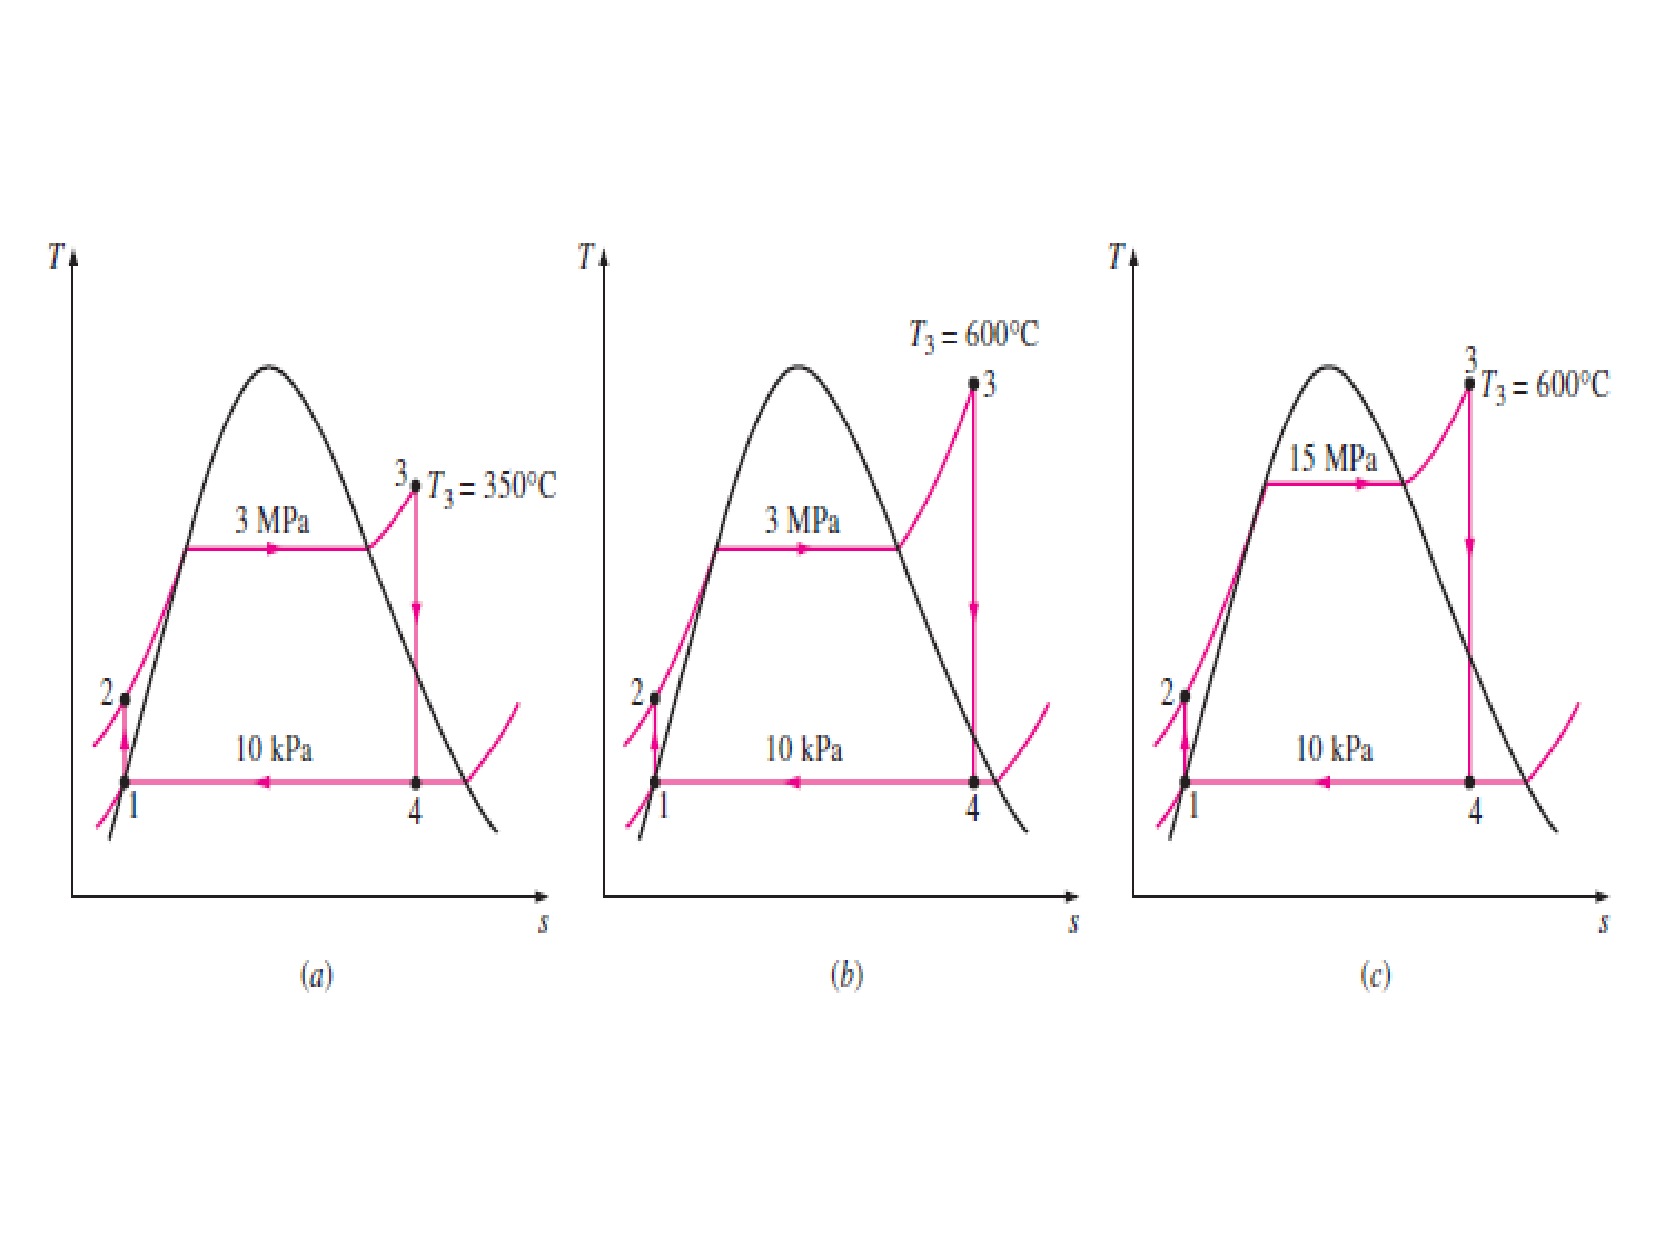
\includegraphics[width=15.0cm,height=9.0cm]{./../../ThermalEngines/Pics/example01_03}
}
\end{center}
\caption{Carnot and Rankine Cycles: Schematic of a Rankine cycle and Ts diagrams -- Example \ref{Example_01_03}.}
\label{Example01_01:Pic3}
\end{figure}

Enthalpy of the fluid leaving the pump can be calculated as
\begin{displaymath}
h_{2}=h_{1}+W_{\text{in}}
\end{displaymath}

where the pump work can be computed as
\begin{displaymath}
W_{\text{in}}=v_{1}\left(P_{2}-P_{1}\right)=3.02\;kJ/kg
\end{displaymath}
therefore the fluid's enthalpy is $h_{2}=194.83\;kJ/kg$. The fluid quality at the turbine output is (assuming isentropic process),
\begin{displaymath}
x_{4}=\frc{s_{4}-s_{f}}{s_{fg}}=\frc{6.7450-0.6492}{7.4996}=0.8128
\end{displaymath}
Thus,
\begin{eqnarray}
&& h_{4}=h_{f}+x_{4}h_{fg}=191.81+0.8128\times 2392.1=2136.1\;kJ/kg \nonumber \\
&& q_{\text{in}}=h_{3}-h_{2}=3116.1-194.83=2921.3\;kJ/kg \nonumber \\
&& q_{\text{out}}=h_{4}-h_{1}=2136.1-191.81=1944.3\;kJ/kg
\end{eqnarray}

and the cycle efficiency is given by,
\begin{displaymath}
\textcolor{blue}{\eta_{\text{(a)}}=1-\frc{q_{\text{out}}}{q_{\text{in}}} = 1 - \frc{1944.3}{2921.3} = 0.334 \text{ or } 33.4\%}
\end{displaymath}

\item \label{example_01_03_b} For this case, phase-states (1) and (2) remain the same whereas the enthapies of (2) and (4) need to be updated

\begin{tabular}{l l l l}
$P_{1}=0.1\;bar$ (saturated liquid) &  $P_{2}=30\;bar$ & $P_{3}=30\;bar$           & $P_{4}=0.1\;bar$ \\
$h_{1}=191.81\;kJ/kg$               &  $s_{2}=s_{1}$   & $T_{3}=873.15\;K$         & $s_{4}=s_{3}$ \\
$v_{1}=1.01\times 10^{-3}\;m^{3}/kg$ &                  & $h_{3}=3682.8\;kJ/kg$     &                 \\
                                    &                 & $s_{3}=7.509\;kJ/(kg.K)$ &                 \\
\end{tabular}

and using the same procedure as Example \ref{example_01_03_a}, $x_{4}=0.915$ and $h_{4}=2380.3\;kJ/kg$. Added and removed heats are
\begin{eqnarray}
&& q_{\text{in}}=h_{3}-h_{2}=3682.8-194.83=3488.0\;kJ/kg \nonumber \\
&& q_{\text{out}}=h_{4}-h_{1}=2380.3-191.81=2188.5\;kJ/kg \nonumber \\
\end{eqnarray}

and the cycle efficiency is given by,
\begin{displaymath}
\textcolor{blue}{\eta_{\text{(b)}}=1-\frc{q_{\text{out}}}{q_{\text{in}}} = 1 - \frc{2188.5}{3488.0} = 0.373 \text{ or } 37.3\%}
\end{displaymath}

The thermal efficiency increases from 33.4$\%$ to 37.3$\%$ (Table \ref{Example01_01:Table2}) as superheated steam temperature is raised from 623.15 K to 873.15 K with a smaller amount of moisture -- from 18.7$\%$ to 8.5 $\%$ (i.e., steam quality increases from 81.3$\%$ to 91.5$\%$).

\item \label{example_01_03_c} For this case, phase-state (1) remain the same but all other phase-states changes. Enthalpies are determined in a similar way as shown in Example \ref{example_01_03_a}: $h_{2}=206.95\;kJ/kg$, $h_{3}=3583.1\;kJ/kg$ and $h_{4}=2115.3\;kJ/kg$ with steam quality as $x_{4}=0.804$.  Added and removed heats then become
\begin{eqnarray}
&& q_{\text{in}}=h_{3}-h_{2}=3583.1-206.95=3376.2\;kJ/kg \nonumber \\
&& q_{\text{out}}=h_{4}-h_{1}=2115.3-191.81=1923.5\;kJ/kg \nonumber \\
\end{eqnarray}

and the cycle efficiency is given by,
\begin{displaymath}
\textcolor{blue}{\eta_{\text{(c)}}=1-\frc{q_{\text{out}}}{q_{\text{in}}} = 1 - \frc{1923.5}{3376.2} = 0.430 \text{ or } 43.0\%}
\end{displaymath}

\medskip


The thermal efficiency increases from 37.3$\%$ to 43.0 $\%$ as the boiler pressure is raised from 30 to 150 bar with constant turbine inlet temperature, 623.15 K (Table \ref{Example01_01:Table2}).

\begin{table}
\begin{center}
\begin{tabular}{c |l l l }
\hline
          &  {\bf Case (a)}      &  {\bf Case (b) }     &  {\bf Case (c) }    \\ 
\hline 
          &   $P_{3}=30\;bar$     &  $P_{3}=30\;bar$     &  $P_{3}=150\;bar$    \\
          &   $T_{3}=623.15\;K$   &  $T_{3}=673.15\;K$   &  $T_{3}=623.15\;K$   \\
          &   $P_{1}=0.1\;bar$    &  $P_{1}=0.1\;bar$    &  $P_{1}=0.1\;bar$    \\
          &   $x_{4}=0.8128$      &   $x_{4}=0.915$      &  $x_{4}=0.804$       \\
\hline
\textcolor{blue}{$\eta \left(\%\right)$} &3\textcolor{blue}{3.4} &\textcolor{blue}{37.3}& \textcolor{blue}{43.0}      \\
\end{tabular}
\end{center}
\caption{Carnot and Rankine Cycles: Improving the efficiency of Rankine cycles, Example \ref{Example_01_03}.}
\label{Example01_01:Table2}
\end{table}



\end{enumerate}

%%%
%%%  Problem 8.2 (SM&VN)
%%%

\item {\it A Carnot engine with water/steam (1 kg/s) as the working fluid operates on the cycle shown in Fig. \ref{PVTSDiags}. For $T_{1}=475\;K$ and $T_{2}=300\;K$, determine: (a) pressures at states 1, 2, 3, and 4; (b) quality $x^{\text{vapour}}$ at states 2 and 3; (c) rate of heat addition; (d) rate of heat rejection; (e) mechanical power for each of the four steps; (f) thermal efficiency $\left(\eta\right)$ of the cycle.}
   \begin{figure}[h]
    \begin{center}
     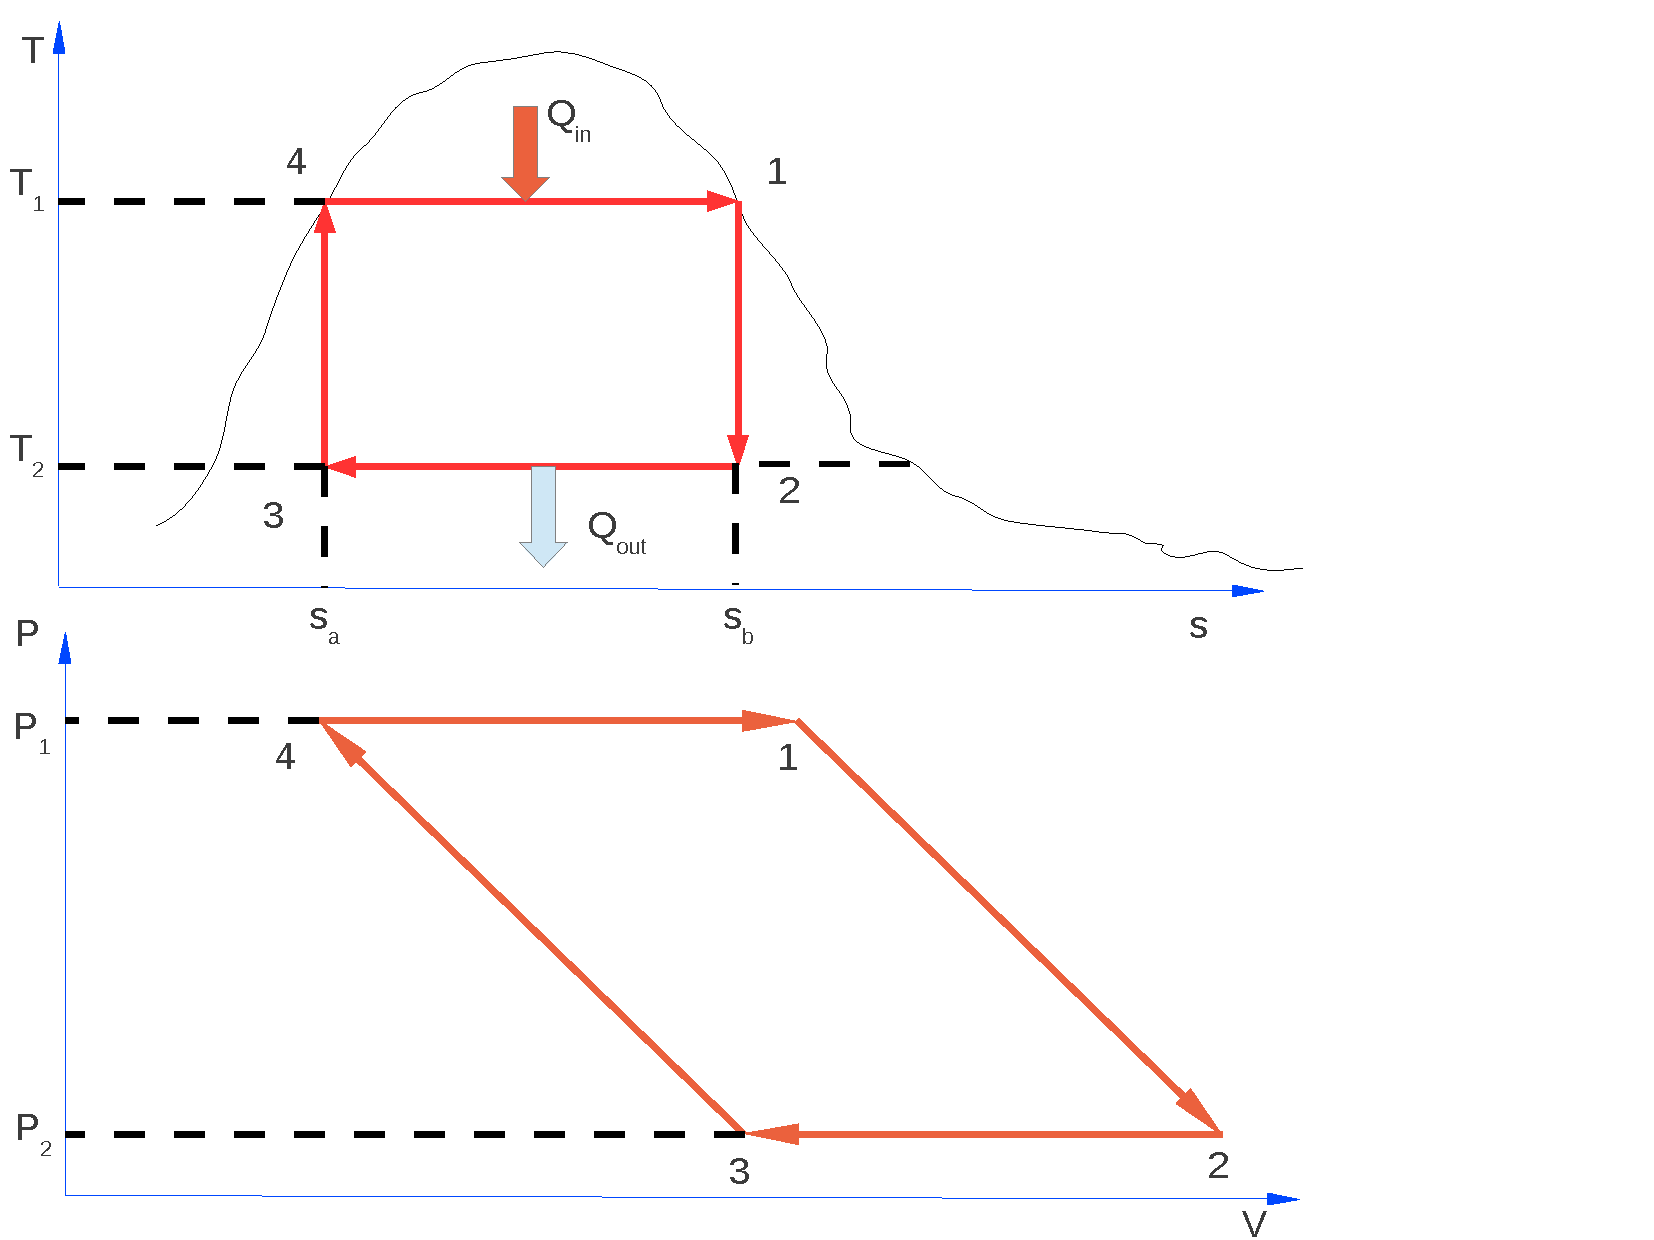
\includegraphics[width=12.cm,clip]{./../../ThermalEngines/Pics/Carnot_PV_TS}
    \end{center}
    \caption{Ts and Pv diagrams for Carnot cycle.}\label{PVTSDiags}
   \end{figure}    

%%%
%%% Problem 8.3 (SM&VN)
%%%
%\item {\it A steam power plant operates on the cycle of Fig. \ref{GenericSteamPlant}. For one of the following sets of operating conditions, determine the steam rate, the heat-transfer rates in the boiler and condenser, and the thermal efficiency of the plant.
%\begin{enumerate}
%\item P1 = P2 = 10000 kPa; T2 = 873.15 K; P3 = P4 = 10     kPa; $\eta_{\text{turbine}}$ = 0.80; $\eta_{\text{pump}}$ = 0.75; power rating = 80  MW.
%\item P1 = P2 = 7000  kPa; T2 = 823.15 K; P3 = P4 = 20     kPa; $\eta_{\text{turbine}}$ = 0.75; $\eta_{\text{pump}}$ = 0.75; power rating = 100 MW.
%\item P1 = Pz = 8500  kPa; T2 = 873.15 K; P3 = P4 = 10     kPa; $\eta_{\text{turbine}}$ = 0.80; $\eta_{\text{pump}}$ = 0.80; power rating = 70  MW.
%\item PI = P2 = 6500  kPa; T2 = 798.15 K; P3 = P4 = 101.33 kPa; $\eta_{\text{turbine}}$ = 0.78; $\eta_{\text{pump}}$ = 0.75; power rating = 50  MW.
%\item P1 = P2 = 7760  kPa; T2 = 866.15 K; P3 = P4 = 7      kPa; $\eta_{\text{turbine}}$ = 0.80; $\eta_{\text{pump}}$ = 0.75; power rating = 80  MW.
%\end{enumerate}
%}
%   \begin{figure}[h]
%    \begin{center}
%     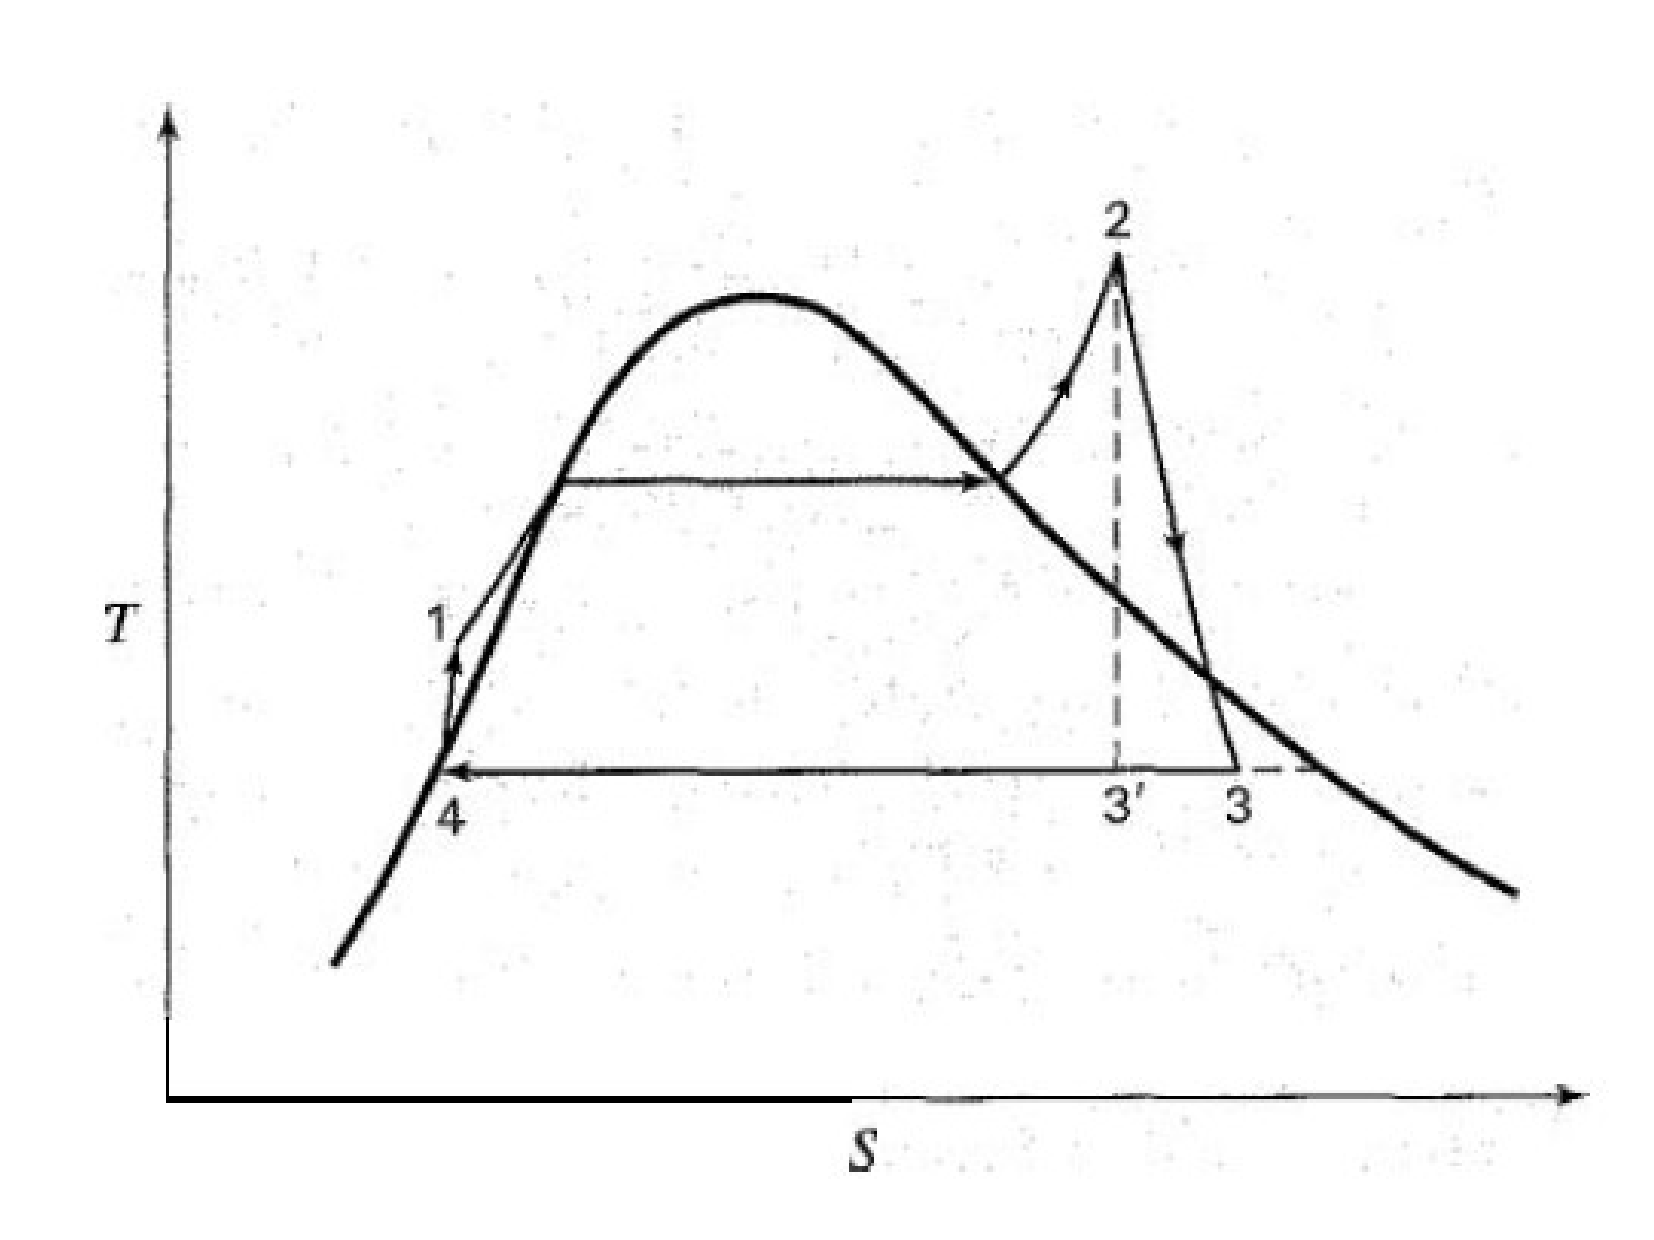
\includegraphics[width=12.cm,clip]{./../../ThermalEngines/Pics/Generic_Steam_Cycle}
%    \end{center}
%    \caption{Generic steam power plant.}\label{GenericSteamPlant}
%     \end{figure}

%%%
%%% Example 12.25 (Rajput)
%%%
\item\label{P:example12_25} {\it A steam power plant operates with with regenerative and reheat arrangement cycles. Steam is supplied to the H.P. turbine (Fig. \ref{example12_25}a) at 80 bar and 470$^{o}$C.  For feed heating, a part of steam is extracted at 7 bar and remainder of the steam is reheated to 350$^{o}$C in a reheater and then expanded in L.P. turbine down to 0.035 bar. Determine: (a) amount of steam bled-off for feed heating; (b) amount of steam supplied to L.P. turbine; (c) heat supplied to the boiler and reheater; (d) cycle efficiency, and (e) power developed by the system. The steam supplied by the boiler is 50 kg/s.}
   \begin{figure}[h]
    \begin{center}
    \vbox{
     \hbox{\hspace{1cm}
      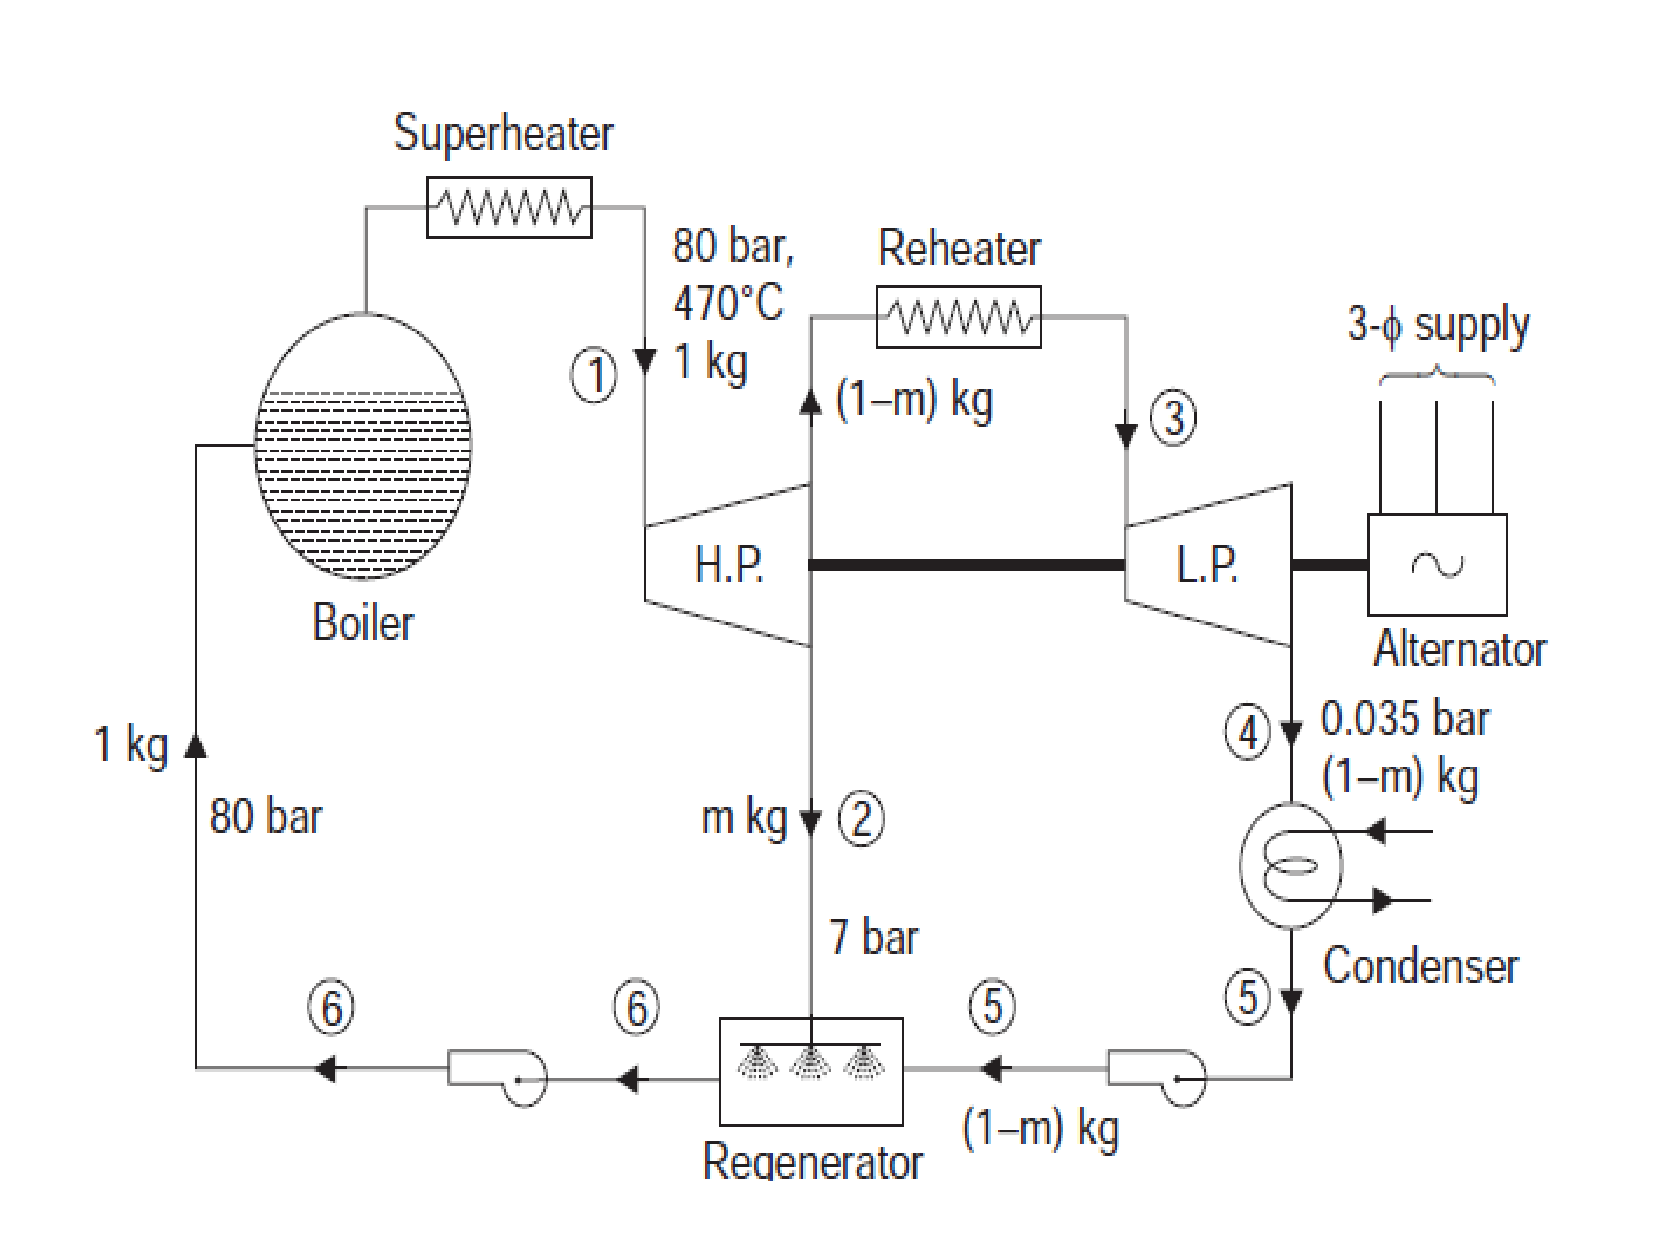
\includegraphics[width=12.cm,clip]{./../../ThermalEngines/Pics/Exemple12_25a_Rajput}}
     \hbox{\hspace{7.5cm}(a)}
     \hbox{\hspace{1.cm}
      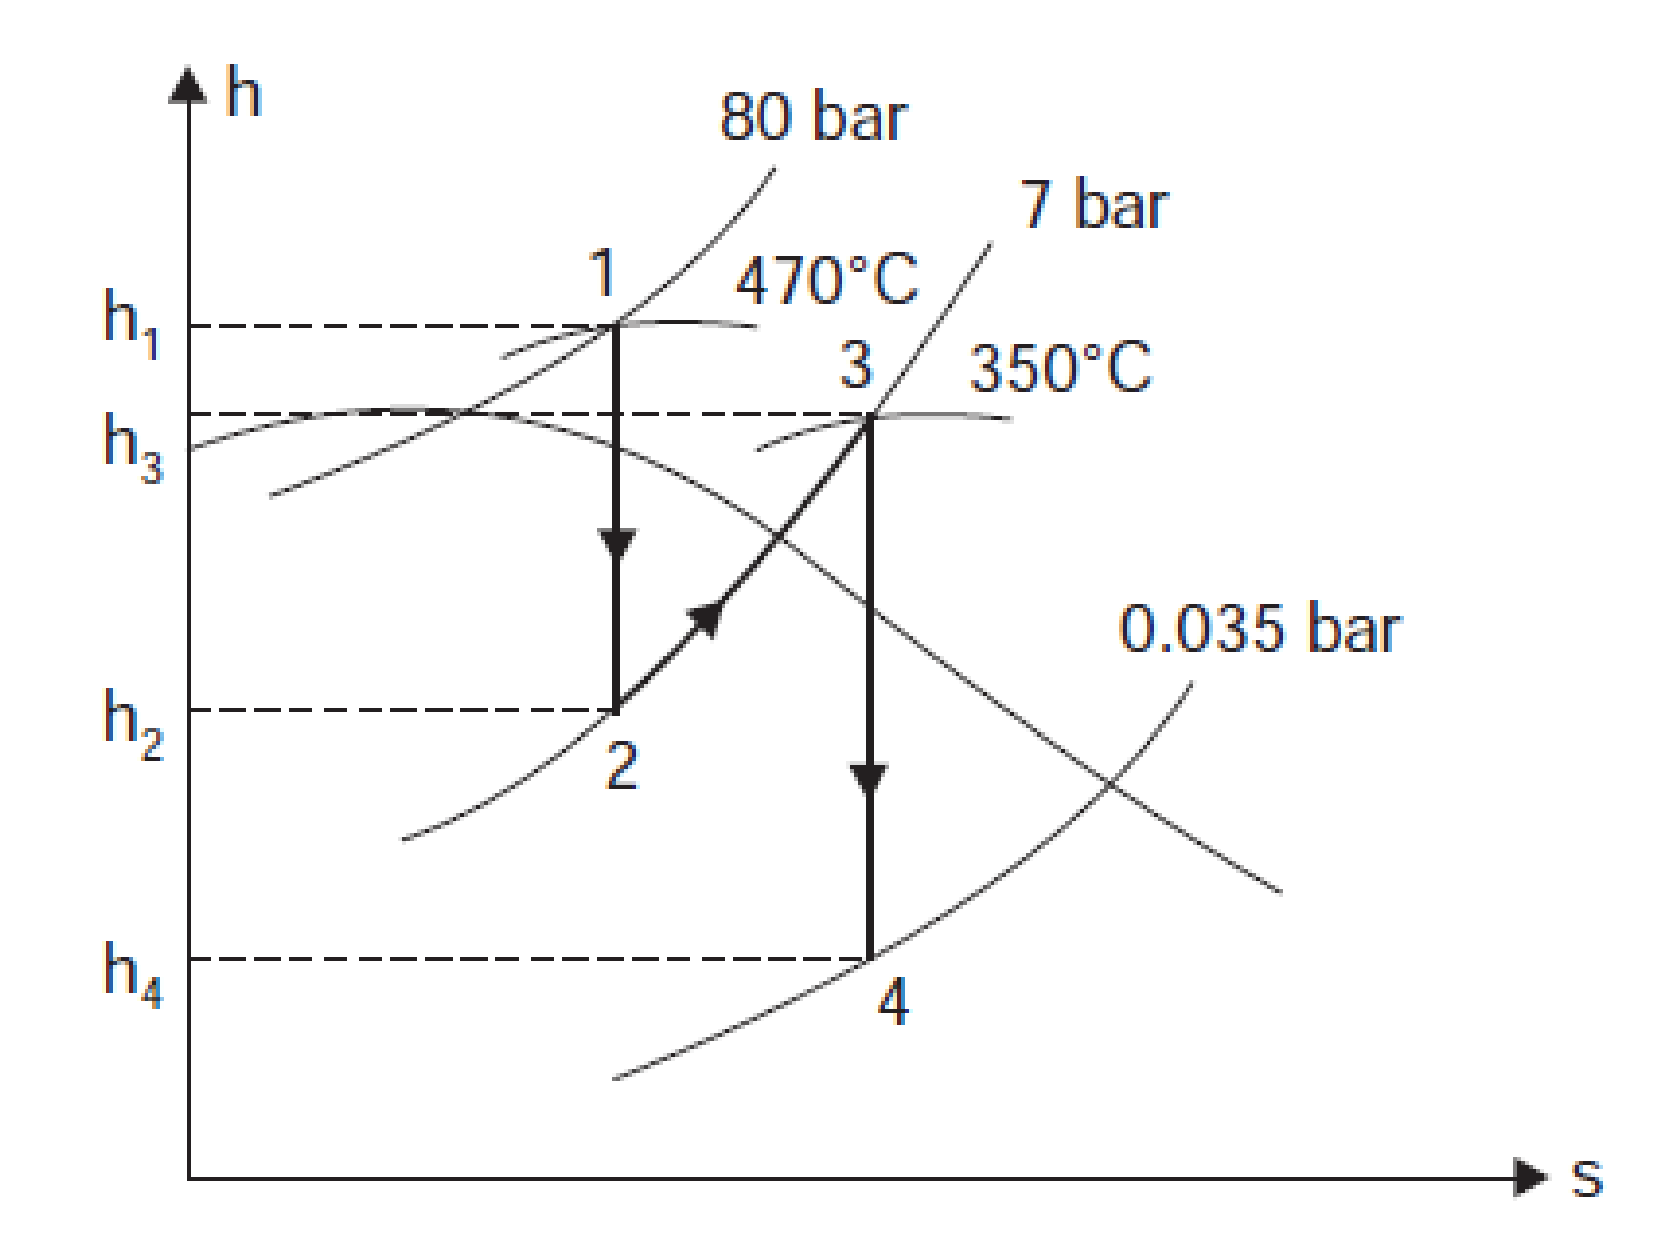
\includegraphics[width=12.cm,clip]{./../../ThermalEngines/Pics/Exemple12_25b_Rajput}
      }
     \hbox{\hspace{7.5cm}(b)}}
     \caption{Problem \ref{P:example12_25}: (a) Schematics and (b) $hs$ diagram of a steam power cycle.}
     \label{example12_25}
     \end{center}
   \end{figure}
 

%%%
%%% Problem 8.6 (Saphiro)
%%%
\item {\it Water is the working fluid in an ideal Rankine cycle. Saturated vapour enters the turbine at 16 MPa, and the condenser pressure is 8 kPa. The mass flow rate of steam entering in the turbine is 120 kg/s. Calculate:
\begin{enumerate}
\item the net power developed (in MW);
\item rate of heat transfer to the steam passing through the boiler (in MW);
\item thermal efficiency;
\item mass flow rate of the condenser cooling water (in kg/s(, if the cooling water undergoes a temperature increase of 18$^{o}$C with negligible pressure change in passing through the condenser.
\end{enumerate} 
}


%%%
%%% Problem 8.12 (Saphiro)
%%%
\item {\it A power plant based on the Rankine cycle is under development to provide a net power output of 10MW. Solar collectors are to be used to generate Refrigerant 22 vapour at 1.6MPa and 50$^{o}$C, for expansion through the turbine. Cooling water is available ar 20$^{o}$C. Specify he preliminary design of the cycle and estimate the thermal efficiency and the refrigerant and cooling water flow rates (in kg/s).}



%%%
%%% Problem 8.16 (Saphiro)
%%%
\item {\it Steam enters the turbine of a simple vapour power plant with a pressure of 10 MPa and temperature $T$, and expands adiabatically to 6 KPa. The isentropuc turbine efficiency is 85$\%$. Saturated liquid exits the condenser at 6KPa and the isentropic pump efficiency is 82$\%$.
\begin{enumerate}
\item For $T=580^{o}$C, determine the turbine exit quality and the cycle thermal efficiency;
\item Compute the same of (a) for $T=700^{o}$C.
\end{enumerate}
}





%%%
%%% Problem 8.6 (SM&VN)
%%%
%\item {\it A steam power plant employs two adiabatic turbines in series. Steam enters the first turbine at 650$^{o}\text{C}$ and 7000 kPa and discharges from the second turbine at 20 kPa. The system is designed for equal power outputs from the two turbines, based on a turbine efficiency of 78$\%$ for each turbine. Determine the temperature and pressure of the steam in its intermediate state between the two turbines. What is the overall efficiency of the two turbines together with respect to isentropic expansion of the steam from the initial to the final state? }

%%%
%%% Problem 8.14 (Saphiro)
%%%
%\item \label{P:problem_lava}{\it On the south coast of the island of Hawaii, lava flows continuously into the ocean. It is proposed to anchor a floating power plant off-shore of the lava flow that uses ammonia as the working fluid. The plant would exploit the temperature variation between the warm water near the surface at 130$^{o}$F and seawater at 50$^{o}$F from a depth of 500 ft to produce power. Figure \ref{problem_lava} shows the configuration and provides additional data. Using the properties of pure water for the seawater and modelling the power as a Rankine cycle, calculate: (a) the thermal efficiency; (b) the mass flow rate of ammonia (in kg/h) for a net output of 300 HP.}
%   \begin{figure}[h]
%    \begin{center}
%      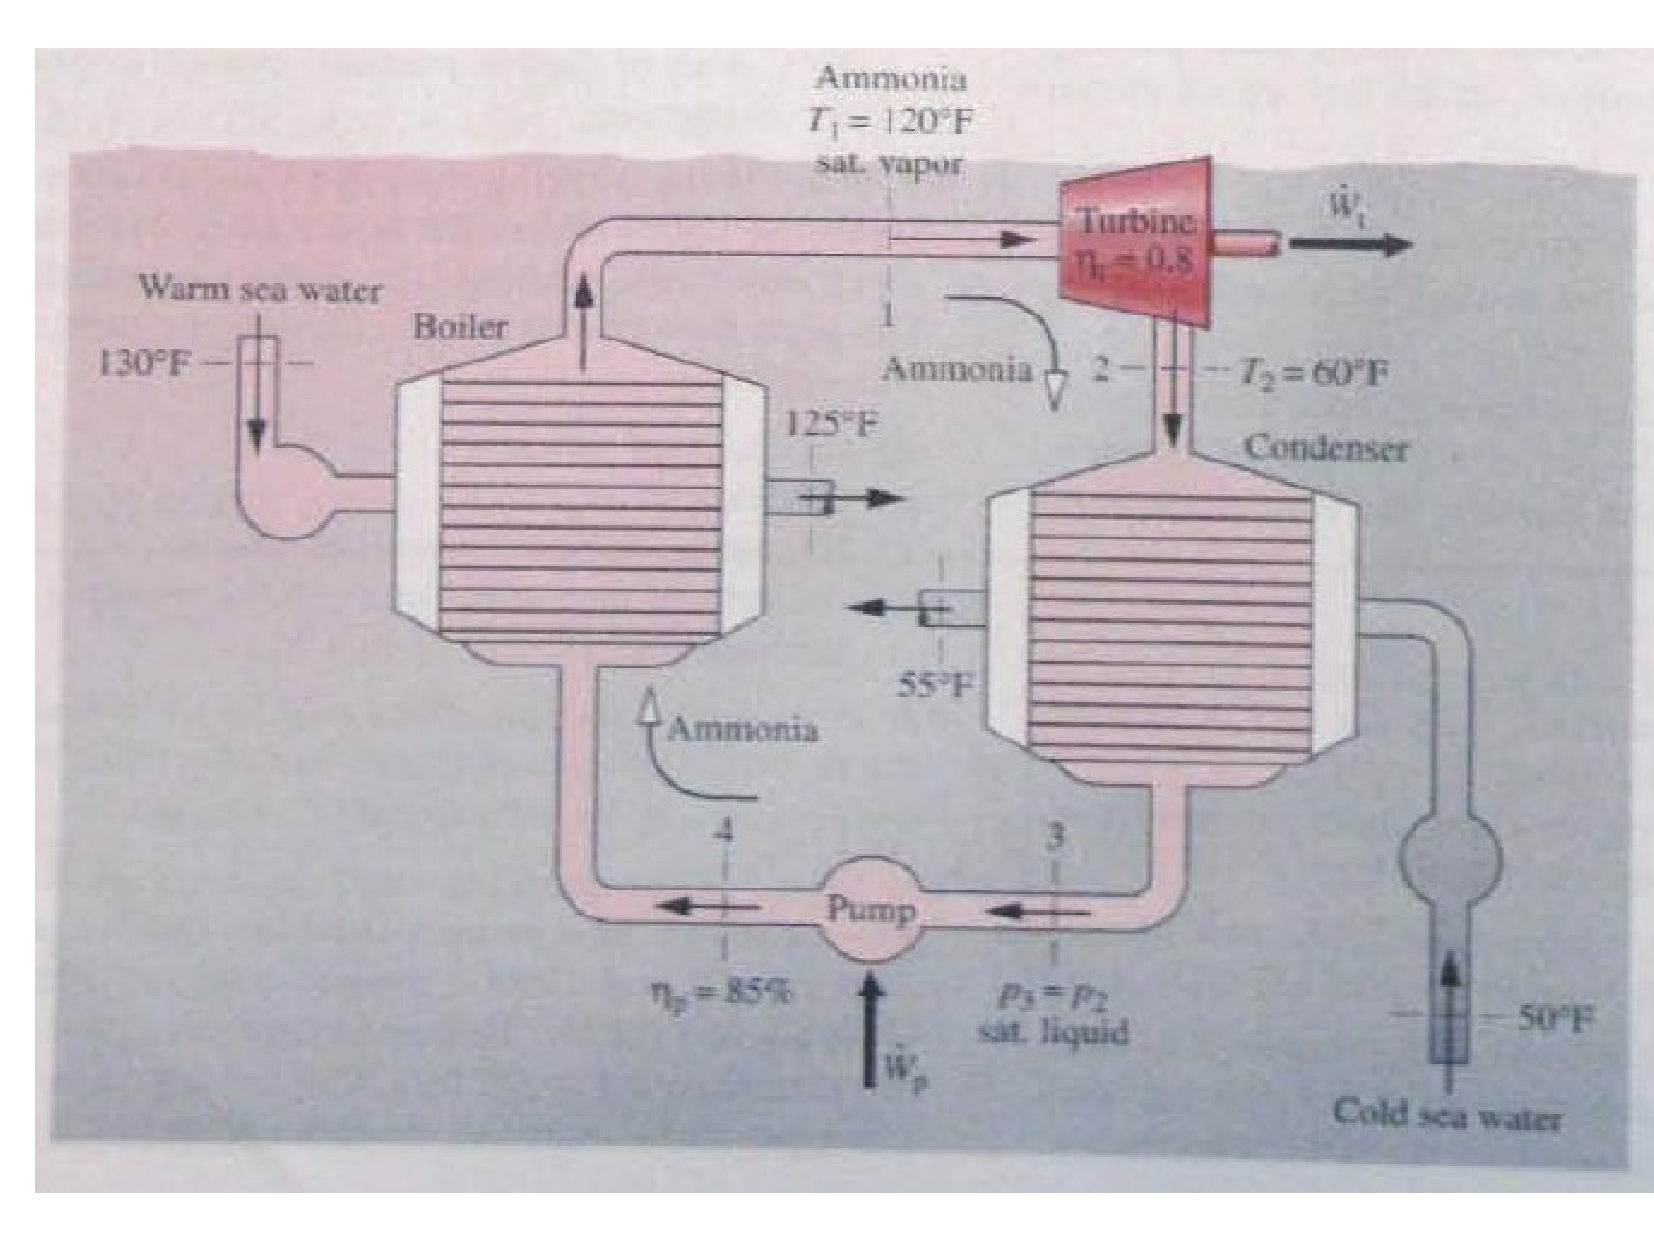
\includegraphics[width=12.cm,clip]{./../../ThermalEngines/Pics/LavaVolcanoPlant}
%     \caption{Problem \ref{P:problem_lava}: Schematics a steam power cycle.}
%     \label{problem_lava}
%     \end{center}
%   \end{figure}


%%%
%%% Problem 8.33 (Saphiro)
%%%
\item {\it Steam at 32 MPa and 520$^{o}$C enters the first stage of a supercritical reheat cycle including three turbine stages. Steam exiting the first-stage turbine at pressure $P$ is reheated at constant pressure to 440$^{o}$C, and steam exiting the second-stage turbine at 0.5 MPa is reheated at constant pressure to 360$^{o}$C.  Each turbine stage and the pump has an isentropic effciency of 85$\%$. The condenser pressure is at 8 kPa. For $P=4\;MPa$, determine the net work per unit mass of steam flowing (kJ/kg) and the thermal efficiency.}


%%%
%%% Problem 8.9 (SM&VN). \ref{example8_9})
%%%
\item \label{P:example8_9}{\it Steam power plant operating on a regenerative cycle, includes just one feedwater heater. Steam enters the turbine at 4500 kPa and 773.15 K and exhausts at 20 kPa. Steam for the feedwater heater is extracted from the turbine at 350 kPa, and in condensing raises the temperature of the feedwater to within 6 K of its condensation temperature at 350 kPa. If the turbine and pump efficiencies are both 0.78, what is the thermal efficiency of the cycle and what fraction of the steam entering the turbine is extracted for the feedwater heater?}



%\item \label{P:example8_9}{\it A steam power plant operating on a regenerative cycle (Fig. \ref{example8_9}), includes two feedwater heaters. Steam enters the turbine at 6500 kPa and 873.15 K and exhausts at 20 kPa. Steam for the feedwater heaters is extracted from the turbine at pressures such that the feedwater is heated to 463.15 K in two equal increments of temperature rise, with 5 K approaches to the steam-condensation temperature in each feedwater heater. If the turbine and pump efficiencies are both 0.80, what is the thermal efficiency of the cycle and what fraction of the steam entering the turbine is extracted for each feedwater heater? }


%\item \label{P:example8_10}{\it A power plant operating on heat recovered from the exhaust gases of internal combustion engines uses isobutane as the working medium in a modified Rankine cycle in which the upper pressure level is above the critical pressure of isobutane. Thus the isobutane does not undergo a change of phase as it absorbs heat prior to its entry into the turbine. Isobutane vapour is heated at 4800 kPa to 533.15 K, and enters the turbine as a supercritical fluid at these conditions. Isentropic expansion in the turbine produces a superheated vapour at 450 kPa, which is cooled and condensed at constant pressure. The resulting saturated liquid enters the pump for return to the heater. If the power output of the modified Rankine cycle is 1000 kW, what is the isobutane flow rate, the heat-transfer rates in the heater and condenser, and the thermal efficiency of the cycle? The vapour pressure of isobutane is given by
%\begin{displaymath}
%\ln\left(P^{\text{sat}}\right) = 1 - \frc{2606.775}{T+0.918}\;\;\;\text{with}\;\;\;\left[P^{\text{sat}}\right]=\text{kPa}\;\;\;\text{and}\;\;\;\left[T\right]=\text{K}
%\end{displaymath}
%Also, the enthalpy of the liquid flows can be obtained from
%\begin{displaymath}
%\Delta H = C_{p}\Delta T + V\left(1-\beta T\right)\Delta P
%\end{displaymath} 
%where
%\begin{displaymath}
%\beta=\frc{1}{V}\left(\frc{\partial V}{\partial T}\right)_{P}
%\end{displaymath}
%is the volume expansivity of fluid.
%}


   %\begin{figure}[h]
   % \begin{center}
   %   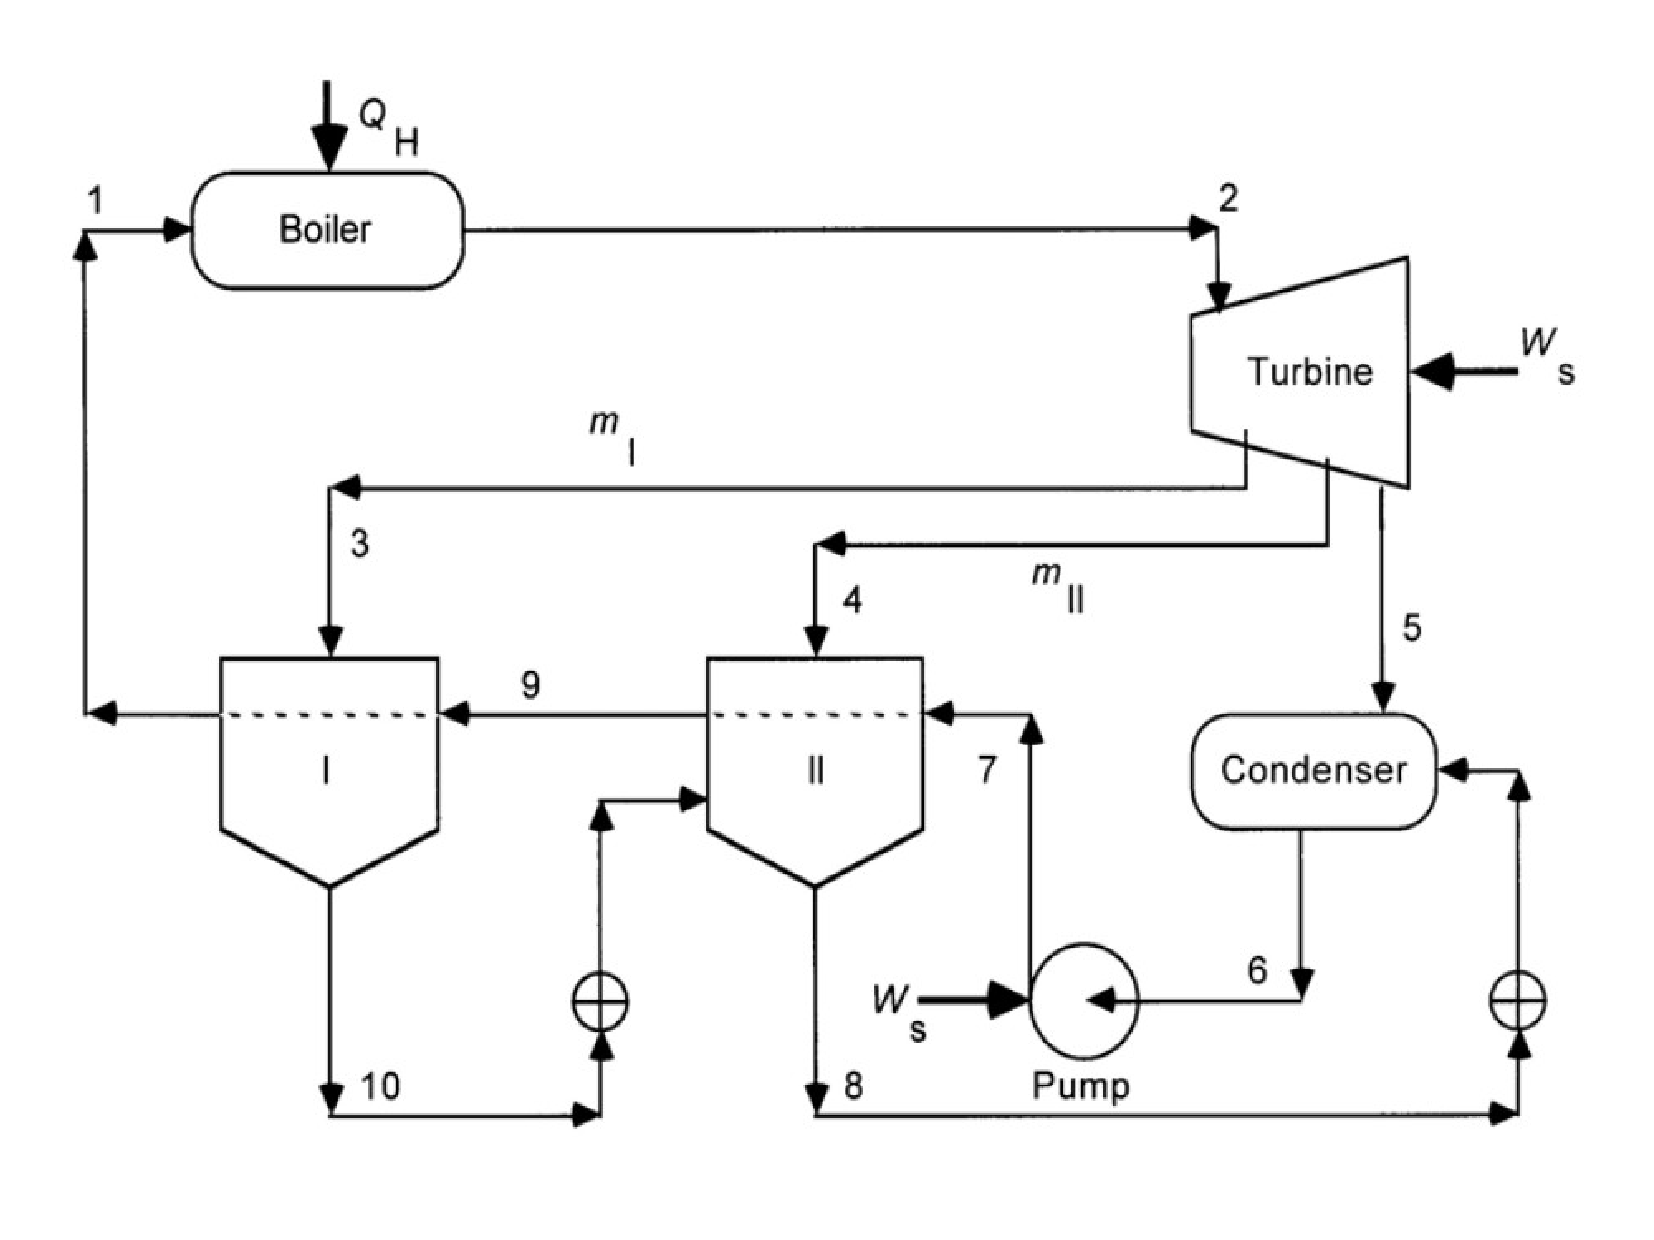
\includegraphics[width=12.cm,clip]{./../../ThermalEngines/Pics/Example_SMVN_8_9}
   %  \caption{Problem \ref{P:example8_9}: Schematics modified Rankine power cycle.}
   %  \label{example8_9}
   %  \end{center}
   %\end{figure}
 


%%%
%%% Problem 8.10 (SM&VN)
%%%
%\item {\it A power plant operating on heat from a geothermal source uses isobutane as the working medium in a Rankine cycle (Fig.\ref{GenericSteamPlant}). Isobutane is heated at 4.8 MPa (a pressure just below its critical pressure) to a temperature of 533.15 K, at which conditions it enters the turbine. Isentropic expansion in the turbine produces superheated vapour at 450 kPa, which is cooled and condensed to saturated liquid and pumped to the heater/boiler. If the flow rate of isobutane is 75 kg/s, what is the power output of the Rankine cycle and what are the heat-transfer rates in the heater/boiler and cooler/condenser? What is the thermal efficiency of the cycle? Repeat these calculations for a cycle in which the turbine and pump each have an efficiency of 80$\%$. The vapour pressure of isobutane is given in Problem \ref{P:example8_9}.}



\end{enumerate}




%\pagebreak

\subsection{Gas Power Systems}

\begin{enumerate}

%%%
%%% Carnot: Example 13.4 (Rajput)
%%%
\item {\it A reversible engine converts one-sixth of the heat input into work. When the temperature of the sink is reduced by 70$^{\text{ o}}$C, its efficiency is doubled. Determine the temperature of the source and the sink.}

Let's first stablish that $T_{1}\text{ and }T_{2}\;\left[\text{K}\right]$ are the source and sink temperatures, respectively. For a {\bf reversible engine}, converting 1/6 of the heat into work means
\begin{displaymath}
\frc{T_{1}-T_{2}}{T_{1}}=\frc{1}{6} \;\;\; \Longrightarrow \;\;\; \textcolor{blue}{T_{1}=1.2T_{2}}
\end{displaymath}
Now if the sink temperature is reduced to {\it 70$^{\text{ o}}$C = 343.15 K}, ie, $T_{2}^{\prime}=T_{2}-343.15$ then the efficiency of the cycle is doubled
\begin{eqnarray}
&& \frc{T_{1}-T_{2}^{\prime}}{T_{1}}=2\times\frc{1}{6} \nonumber \\
&& 2T_{1}=3T_{2}-1029.45\;\;\Longrightarrow\;\;T_{2}=1715\text{ K and }T_{1}=2058.90\text{ k}\nonumber
\end{eqnarray}

%%%
%%% Carnot: Example 13.6 (Rajput)
%%%
\item {\it An ideal engine operates on the Carnot cycle using a perfects gas as the working fluid. The ratio of the greatest to the least volume is fixed as $x : 1$, the lower temperature of the cycle is also fixed, but the volume compression ratio $r$ of the reversible adiabatic compression is variable. The ratio of the specific heats is $\gamma$. Show that if the work done in the cycle is a maximum then,
\begin{displaymath}
  \left(\gamma-1\right)\ln\frc{x}{r}+\frc{1}{r^{\gamma-1}}-1=0
\end{displaymath}
}

%%%
%%% Otto: Example 13.9 (Rajput)
%%%
\item {\it The minimum pressure and temperature in an Otto cycle are 100 kPa and 27 $^{\text{ o}}$C. The amount of heat added to the air per cycle is 1500 kJ/kg. Calculate:
\begin{enumerate}
\item Pressures and temperatures at all stages of the air standard Otto cycle;
\item Specific  work and thermal efficiency of the cycle for a compression ratio of 8 : 1.
\end{enumerate}
}
Assuming an isentropic compression stage 1--2 and an isentropic expansion stage 3--4 with a compression ratio $V_{1}/V_{2}= 8$. Initial temperature of 300.15 K and pressure of 100 kPa.
\begin{itemize}
%
\item {\it adiabatic compression (1--2):}
\begin{displaymath}
  \frc{T_{2}}{T_{1}}=\left(\frc{V_{1}}{V_{2}}\right)^{\gamma-1}=r^{\gamma-1}=8^{1.4-1}=2.297\;\;\Longrightarrow\;\;T_{2}=689.10\text{ K}
\end{displaymath}
and
\begin{displaymath}
\frc{P_{1}}{P_{2}}=\left(\frc{V_{1}}{V_{2}}\right)^{\gamma}=18.379\;\Longrightarrow P_{2}=18.379\text{ bar}
\end{displaymath}

\item {\it constant volume (2--3):} heat added: $C_{v}\left(T_{3}-T_{2}\right)=1500\Longrightarrow T_{3}=2772.4\text{ K}$ and 
\begin{displaymath}
\frc{P_{2}}{T_{2}}=\frc{P_{3}}{T_{3}}\Longrightarrow P_{3}=73.94\text{ bar}
\end{displaymath}

\item {\it adiabatic expansion (3--4):}
\begin{displaymath}
\frc{T_{3}}{T_{4}}=\left(\frc{V_{4}}{V_{3}}\right)^{\gamma-1}=r^{\gamma-1}\;\Longrightarrow T_{4}=1206.9\text{ K}
\end{displaymath}
and
\begin{displaymath}
P_{3}V_{3}^{\gamma}=P_{4}V_{4}^{\gamma}\;\Longrightarrow P_{4}=4.023\text{ bar}
\end{displaymath}

\item {\it Specific work} = heat added - heat rejected
\begin{displaymath}
W= C_{v}\left(T_{3}-T_{2}\right)-C_{v}\left(T_{4}-T_{1}\right)=847\text{ kJ/kg}
\end{displaymath}

\item {\it Thermal efficiency:}
\begin{displaymath}
\eta_{\text{Otto}}=1- \frc{1}{r^{\gamma-1}} = 0.5647
\end{displaymath}
%
\end{itemize}


%%%
%%% Otto: Example 13.10 (Rajput)
%%%
\item {\it An ideal Otto cycle has a volumetric compression ratio of 6, the lowest cycle pressure of 0.1 MPa and operates between temperature limits of 300.15 and 1842.15 K.
\begin{enumerate}
\item \label{a}Calculate the temperature and pressure after the isentropic expansion;
\item Since the values in (\ref{a}) are well above the lowest cycle operating conditions, the expansion process was allowed to continue down to a pressure of 0.1 MPa. Which process is required to complete the cycle ? 
\item  Determine the percentage in which the cycle efficiency has improved.
\end{enumerate}
}

%%%
%%% Otto: Example 13.12 (Rajput)
%%%
%\item {\it In a constant volume Otto cycle, the pressure at the end of compression stroke is 15 times that at the start. The temperature of air at the beginning of compression is 38 $^{\text{ o}}$C and maximum temperature attained in the cycle is 1950 $^{\text{ o}}$C. Calculate: (i) compression ratio; (ii) thermal efficiency of the cycle and (iii) work done.}


%%%
%%% Diesel: Example 13.22 (Rajput)
%%%
\item {\it The volume ratios of compression and expansion for a diesel engine are 15.3 and 7.5, respectively. The pressure and temperature at the beginning of the compression are 1 bar and 27 $^{\text{ o}}$C. Assuming an ideal engine, determine the (a) MEP, (b) ratio of maximum pressure to MEP and (c) cycle efficiency. Also find the fuel consumption per kWh if the indicated thermal efficiency is 0.5 of ideal efficiency, mechanical efficiency is 0.8 and the calorific value of oil 42000 kJ/kg. }


%%%
%%% Dual: Prob 9.33 (Saphiro) 
%%%
%\item {\it An air-standard dual cycle has a compression ratio of 9. At the beginning of compression, $P_{1}=100\text{ kPa}$, $T_{1}=300\text{ K}$ and $V_{1}=14\text{ liters}$. The heat addition is 22.7 KJ with one-half added at constant volume and one-half added at constant pressure. Determine: (a) the temperatures at the end of each heat addition process; (b) the net work of the cycle per unit mass of air; (c) the thermal efficiency and; (d) MEP.}

\end{enumerate}


\setcounter{page}{1}
\pagenumbering{roman}
%\begin{appendix}
%
\section{Introduction to Partial Differentiation}
Eight properties of a system -- pressure ({\it P}), volume ({\it V}), temperature ({\it T}), internal energy ({\it u}), enthalpy ({\it h}), entropy ({\it s}), Helmholtz free energy ({\it f}) and Gibbs free energy ({\it g}) have been introduced in EG2004 (Fluid Mechanics and Thermodynamics) and EG3020 (Process Thermodynamics). {\it h}, {\it f} and {\it g} are sometimes referred to as thermodynamic potentials. Both {\it f} and {\it g} are extremely important when considering chemical reactions (e.g., combustion) and processes involving phase change (e.g., water/steam industrial systems, atmospheric and crystallisation processes etc).

From the aforementioned (eight) properties, only pressure, temperature and volume can be directly measurable. Therefore it is convenient to introduce other combination of properties which are relatively easily measurable and which, along with {\it P}, {\it T} and {\it V}, enable the values of the remaining properties to be determined. These combinations of properties are commonly referred as {\it thermodynamic gradients} -- i.e., they are defined as the rate of change of one property with another while a third is kept constant.

\medskip

Let's consider three variables $x$, $y$ and $z$, and their functional relationship, $f\left(x,y,z\right)=0$ with $x=x(y,z)$, $y=y(x,z)$ and $z=z(x,y)$.  The intrinsic relationship of the differential dependent variable $x=x(y,z)$ in relation to the independent variables $y$ and $z$ can be represented as
\begin{equation}
dx = \left(\frc{\partial x}{\partial y}\right)_{z}dy + \left(\frc{\partial x}{\partial z}\right)_{y}dz
\label{exact_diff_dx}
\end{equation}
\noindent
in which $dx$ is the exact differential. Renaming $M=\left(\frc{\partial x}{\partial y}\right)_{z}$ and $N=\left(\frc{\partial x}{\partial z}\right)_{y}$, and Eqn. \ref{exact_diff_dx} can be rewritten as,
\begin{equation}
dx = Mdy + Ndz \label{diff1}
\end{equation}
\noindent
The partial differentiation of $M$ and $N$ with respect to $z$ and $y$, respectively, leads to,
\begin{equation}
  \frc{\partial M}{\partial z}=\frc{\partial^{2} x}{\partial y \partial z} \;\;\;\text{and}\;\;\; \frc{\partial N}{\partial y}=\frc{\partial^{2} x}{\partial z \partial y} \;\; \Longleftrightarrow \;\;  \frc{\partial M}{\partial z}=\frc{\partial N}{\partial y} \label{diff2}
\end{equation}
\noindent
Similarly for $y=y(x,z)$ and $z=z(x,y)$, 
\begin{eqnarray}
  dy = \left(\frc{\partial y}{\partial x}\right)_{z}dx + \left(\frc{\partial y}{\partial z}\right)_{x}dz \nonumber \\
  dz = \left(\frc{\partial z}{\partial x}\right)_{y}dx + \left(\frc{\partial z}{\partial y}\right)_{x}dy \nonumber
\end{eqnarray}
\noindent
Replacing $dz$ in $dy$ above,
\begin{eqnarray}
dy &=& \left(\frc{\partial y}{\partial x}\right)_{z}dx +  \left(\frc{\partial y}{\partial z}\right)_{x} \left[ \left(\frc{\partial z}{\partial x}\right)_{y}dx + \left(\frc{\partial z}{\partial y}\right)_{x}dy \right] \nonumber \\
%
  &=& \left[ \left(\frc{\partial y}{\partial x}\right)_{z} + \left(\frc{\partial y}{\partial z}\right)_{x} \left(\frc{\partial z}{\partial x}\right)_{y} \right]dx + dy \nonumber 
\end{eqnarray}
\noindent
Clearly, the term in the square-brackets vanishes,
\begin{eqnarray}
&& \left(\frc{\partial y}{\partial x}\right)_{z} + \left(\frc{\partial y}{\partial z}\right)_{x} \left(\frc{\partial z}{\partial x}\right)_{y}  = 0 \nonumber \\
%
&& \left(\frc{\partial y}{\partial z}\right)_{x} \left(\frc{\partial z}{\partial x}\right)_{y} =  -\left(\frc{\partial y}{\partial x}\right)_{z} \nonumber \\
&&  \left(\frc{\partial x}{\partial y}\right)_{z} \left(\frc{\partial z}{\partial x}\right)_{y} \left(\frc{\partial y}{\partial z}\right)_{x} = -1 \label{diff3}
\end{eqnarray}
\noindent
Replacing $x$, $y$ and $z$ by $P$, $V$ and $T$,
\begin{equation}
\left(\frc{\partial P}{\partial V}\right)_{T} = \left(\frc{\partial T}{\partial P}\right)_{V} = \left(\frc{\partial V}{\partial T}\right)_{P} = -1
\end{equation}

\section{Thermodynamic Relations}

From the Course Notes we saw that the First Law applied to a closed system in a reversible process states that,
\begin{equation}
dQ= du + PdV, \label{firstlaw_simplified}
\end{equation}
\noindent
and the Second Law,
\begin{equation}
ds=\left(\frc{dQ}{T}\right)_{\text{rev}}
\end{equation}
\noindent
we can combine these equations to obtain
\begin{equation}
du = - PdV + Tds \label{gibbs_eqn0}
\end{equation}
We can similarly derive the equations for enthalpy, free Gibbs and free Helmholtz energy equations as
\begin{eqnarray}
&& dh = Tds + VdP \label{enthalpy_eqn} \\
&& df = -PdV - sdT \label{helmholtz_eqn} \\
&& dg = -VdP -sdT \label{gibbs_eqn}
\end{eqnarray}

\noindent
As $du$, $dh$, $df$ and $dg$ are exact differentials, we can express them as the following set of chain rule -based differentials,
\begin{eqnarray}
du = \left(\frc{\partial u}{\partial  s}\right)_{V}ds + \left(\frc{\partial u}{\partial V}\right)_{s}dV \nonumber \\
%
dh = \left(\frc{\partial h}{\partial  s}\right)_{P}ds + \left(\frc{\partial h}{\partial P}\right)_{s}dP \nonumber \\
%
df = \left(\frc{\partial f}{\partial  V}\right)_{T}dV + \left(\frc{\partial f}{\partial T}\right)_{V}dT \nonumber \\
%
dg = \left(\frc{\partial g}{\partial  P}\right)_{T}dP + \left(\frc{\partial g}{\partial T}\right)_{P}dT \nonumber \\
\end{eqnarray}


\section{Maxwell Relations}

Comparing the Gibbs equation (\ref{gibbs_eqn0}) with Eqn. \ref{diff1} for $dx$,
\begin{displaymath}
du = -PdV +Tds \;\;\;\;\;\text{and}\;\;\;\;\; dx = Mdy + Ndz 
\end{displaymath}
We can easily notice the mathematical equivalences,
\begin{displaymath}
x\Longrightarrow u, \;\; y\Longrightarrow V, \;\; z\Longrightarrow s, \;\; M\Longrightarrow -P, \;\; N\Longrightarrow T
\end{displaymath}
\noindent
With the analogy of $x=x(y,z)$ and $u=u(V,s)$, Eqn. \ref{diff2} leads to,
\begin{equation}
-\left(\frc{\partial P}{\partial s}\right)_{V} = \left(\frac{\partial T}{\partial V}\right)_{s}, \label{maxwell_rel1} 
\end{equation}
\noindent
$\left(\frc{\partial u}{\partial V}\right)_{s} = -P$ and $\left(\frc{\partial u}{\partial s}\right)_{V}=T$.  Eqn. \ref{maxwell_rel1} is known as a {\it Maxwell relation}. Similar relations can be obtained from the remaining fundamental thermodynamics equations -- Eqns. \ref{enthalpy_eqn}-\ref{gibbs_eqn} leading to the whole set of {\it Maxwell relations}:
\begin{eqnarray}
%
 \left(\frac{\partial T}{\partial V}\right)_{s} &=& -\left(\frc{\partial P}{\partial s}\right)_{V} \nonumber \\
%
 \left(\frc{\partial T}{\partial P}\right)_{s} &=& \left(\frac{\partial V}{\partial s}\right)_{P} \label{maxwell_rel2} \\
%
 \left(\frc{\partial P}{\partial T}\right)_{V} &=& \left(\frac{\partial s}{\partial V}\right)_{T} \label{maxwell_rel3} \\
%
  \left(\frac{\partial V}{\partial T}\right)_{P} &=& -\left(\frc{\partial s}{\partial P}\right)_{T} \label{maxwell_rel4} 
\end{eqnarray}
\noindent
with,
\begin{eqnarray}
%
\left(\frc{\partial u}{\partial s}\right)_{V} & =  T  = & \left(\frc{\partial h}{\partial s}\right)_{P} \label{maxwell_coef1} \\
%
\left(\frc{\partial u}{\partial V}\right)_{s} & = - P = & \left(\frc{\partial f}{\partial V}\right)_{T} \label{maxwell_coef2} \\
%
\left(\frc{\partial h}{\partial P}\right)_{s} & =  V =  & \left(\frc{\partial g}{\partial P}\right)_{T} \label{maxwell_coef3} \\
%
\left(\frc{\partial f}{\partial T}\right)_{V} & =  -s  = & \left(\frc{\partial g}{\partial T}\right)_{P} \label{maxwell_coef4}
%
\end{eqnarray}

Equations \ref{maxwell_rel1}-\ref{maxwell_coef4} do not refer to a process, but do express relations between properties which must be satisfied when any system is in a state of equilibrium.




%\end{appendix}

\end{document}
